\documentclass[oneside]{arco-pfc}
\usepackage{custom}
\usepackage{metadata}
\usepackage{eurosym} % para el euro
\usepackage{multirow} % para las tablas
\usepackage{hyperref}
\usepackage{pdfpages}

\newcommand{\vcenteredinclude}[1]{\begingroup
\setbox0=\hbox{\includegraphics{#1}}%
\parbox{\wd0}{\box0}\endgroup}



%----------------------------------------------------------------------------------------
%	TITLE PAGE
%----------------------------------------------------------------------------------------

\newcommand*{\rotrt}[1]{\rotatebox{90}{#1}} % Command to rotate right 90 degrees
\newcommand*{\rotlft}[1]{\rotatebox{-90}{#1}} % Command to rotate left 90 degrees

\newcommand*{\titleBC}{\begingroup % Create the command for including the title page in the document
\centering % Center all text
\vfill
\def\CP{\textit{\Huge Quercus Pyrenaica}} % Title

\settowidth{\unitlength}{\CP} % Set the width of the curly brackets to the width of the title
{\color{LightGoldenrod}\resizebox*{\unitlength}{\baselineskip}{\rotrt{$\}$}}} \\[\baselineskip] % Print top curly bracket
\textcolor{Sienna}{\CP} \\[\baselineskip] % Print title
{\color{RosyBrown}\Large Plan de Empresa} \\ % Tagline or further description
{\color{LightGoldenrod}\resizebox*{\unitlength}{\baselineskip}{\rotlft{$\}$}}} % Print bottom curly bracket
\vfill
\begin{figure}[h]
  \begin{center}
    
\includegraphics[scale=0.4]{logos/borrador1.png}
  \end{center}
\end{figure}
\vfill % Whitespace between the title and the author name

{\Large\textbf{Jesús Burgos Plaza}}\\ % Author name
\vfill % Whitespace between the author name and the publisher logo

Escuela Superior de Gastronomía Y Hostelería de Toledo\\
Febrero de 2014 % Year published

\endgroup}

\begin{document}

\pagestyle{empty} % Removes page numbers

\titleBC



\frontmatter

%\input{resumen.tex}
%\input{abstract.tex}

\tableofcontents
%\listoftables
\listoffigures
\listoftables
%\lstlistoflistings
%\input{acronimos.tex}
%\input{agradecimientos.tex}
\dedication{"La responsabilidad del cocinero está enfocada al respeto de los recursos del planeta y de consumirlos de manera sostenible.
Intentar usar los pescados más sostenibles, consumir menos proteína animal, más cereal, enfocarse más en la nutrición. 
Y por la salud del consumidor, intentar comer menos sal, menos grasa y menos azúcar. Ser lo más cercano a la naturaleza".
\\ Alain Ducasse }


\mainmatter
%\pagestyle{empty} % Removes page numbers

\titleBC


\chapter{Presentación del proyecto}
\label{chap:presentacion}

El objetivo principal es poner en marcha un complejo con bungalows y un restaurante vegetariano con productos ecológicos y de temporada, para hacer frente a la creciente demanda en el sector de \emph{clientes verdes}, denominando así, de forma escueta, a todos aquellos clientes que van  buscando cierta calidad en los productos, al no ser tratados con herbicidas ni pesticidas y por no ser de origen transgénico.

Como objetivo secundario, se pretende impartir clases de cocina a grupos de personas que quieran aprender a cocinar y cultivar estos productos por cuenta propia para llegar a ser un poco más autosuficiente.

\section{Justificación}
\label{sec:justificacion}
La idea de este negocio, surge a partir de mis dos grandes pasiones en esta vida: la cocina y el medio ambiente, y poder poner en práctica mis dos titulaciones que son Dirección de Cocina y Técnico Superior en la Gestión y Organización de los Recursos Naturales y Paisajísticos. Pudiendo así combinarlas en mi trabajo y realizarme como persona.

\section{Datos básicos de la empresa}
\label{sec:datos}
%Datos básicos: nombre, localización de la empresa

La empresa se encuentra situada en las afueras del término municipal de Poyales del Hoyo, en la provincia de Ávila.
Las coordenadas UTM de la ubicación exacta son:

X = 315.457.82 m

Y = 4.449.536.18 m

En la Figura \ref{fig:plano} se muestra dicha ubicación sobre el plano de la zona.

\begin{figure}[h]
  \begin{center}
    \includegraphics[scale=0.6]{images/plano.jpg}
    \caption{Ubicación de la empresa}
    \label{fig:plano}
  \end{center}
\end{figure}

El nombre de la empresa, \textbf{\textit{Quercus pyrenaica}}, viene a representar  una de las especies más abundantes que se encuentran a esta altura, de la familia \emph{Fagaceae}. Este género es uno de los más representativos dentro de la vegetación en la península ibérica.

La forma jurídica elegida para esta empresa es una sociedad limitada nueva empresa, cuyo nombre va a ser \emph{Jesús Burgos Plaza A2E45 SLNE}. Cuyo único socio es Jesús Burgos Plaza, con un capital mínimo de constitución de 3012 \euro. Siendo el 100\% de las acciones del único socio. 

El terreno procede de una herencia familiar, donde ya se encontraba ubicado un restaurante acondicionado con todas las instalaciones necesarias para poder continuar con la actividad. Gracias a esto, solo ha sido necesaria la compra de los bungalows para poder cambiar de categoría de restaurante a complejo hostelero. Los bungalows adquiridos son prefabricados, de manera que únicamente ha habido que instalarlos sobre el terreno. Siendo el precio de los de capacidad para cuatro personas de 50.000\euro y los de capacidad para dos de 28.000\euro.

El logotipo de la empresa es el que se muestra en la Figura \ref{fig:logo}.

\begin{figure}[htb]
  \begin{center}
    
\includegraphics[scale=0.4]{logos/borador2.png}
    \caption{Logotipo de la empresa}
    \label{fig:logo}
  \end{center}
\end{figure}

\section{Identificación del socio}
\label{sec:identificacion}

Los clientes a los que va dirigido este complejo hostelero son personas que están concienciadas del medio ambiente, que quieran aprender de los cursos que se imparten desde las instalaciones o disfrutar de éstas, tanto en el restaurante como de los bungalows, además de disfrutar de las maravillosas vistas del entorno en el que está localizado el complejo y de otras actividades que se pueden realizar por la comarca.

Para poder dar los mejores servicios a nuestros clientes, la carta de presentación del socio es la que se muestra en el Cuadro \ref{tab:cartaPresentacion}.

% Please remember to add \use{multirow} to your document preamble in order to suppor multirow cells
\begin{table}[h]
\begin{tabular}{|l|lllll}
\cline{1-2}
Nombre: Jesús Burgos Plaza                                                                                                            & Edad: 29 años                                                                                                           & \multicolumn{4}{l}{\multirow{3}{*}{}} \\ \cline{1-2}
\multicolumn{2}{|l|}{\begin{tabular}[l]{@{}l@{}}Formación:\\ - Técnico Superior en la Gestión y Organización de los Recursos Naturales y Paisajísticos.\\ - Técnico Superior en Dirección de Cocina.\end{tabular}}                                                  & \multicolumn{4}{l}{}                  \\ \cline{1-2}
\multicolumn{2}{|l|}{\begin{tabular}[l]{@{}l@{}}Con experiencia en los dos sectores. Habiendo trabajado para la empresa \emph{Tragsa}\\ en varios puestos relacionados con el sector forestal y con prácticas en el restaurante\\ vegetariano \emph{Madre Tierra}.\end{tabular}} & \multicolumn{4}{l}{}                  \\ \cline{1-2}
\multicolumn{2}{l}{}                                                                                                                                                                                                                                            &         &         &         &        
\end{tabular}
\caption{Carta de presentación del socio}
\label{tab:cartaPresentacion}
\end{table}

Existe un espíritu emprendedor, ganas de llevar hacia delante el proyecto y que  permita desarrollar las capacidades adquiridas con la formación académica.

\section{Objetivos para conseguir}
\label{sec:objetivos}

\begin{itemize}
\item Facilitar a los clientes la adquisición de conocimientos forestales y agrícolas para poder ser más autosuficientes.
\item Ofrecer servicios de alojamiento y de restauración con la mayor calidad posible.
\item Fomentar la participación de nuestros mismos clientes.
\item Informar a los clientes de todas aquellas actividades que puede realizar por la zona. Para ello, varias empresas de la comarca nos hemos juntado para hacer un Stakeholder, en el cual, colaboramos entre todos, dándonos nosotros  mismos publicidad entre todas las empresas que formamos parte (Granja Escuela Casavieja, campamento parque de cuerdas, Casavieja,La Colonia de Gredos; granja escuela centro de naturaleza, Candeleda, Casa del Parque El Risquillo; centro de interpretación, Guisando; Turismo Ecuestre en el Valle del Tiétar sur de Gredos, Cabalgando en Gredos, rutas - turismo ecuestre, Arenas de San Pedro; Club Hípico Roble Alto, turismo ecuestre, Candeleda; Gredos Ecuestre, rutas - turismo ecuestre, Arenas de San Pedro; La Espuela Centro Ecuestre, La Adrada
\end{itemize}


\newpage
\section{Análisis DAFO}
\label{sec:dafo}

Mediante este análisis se pretende hacer una valoración general del proyecto, analizando las Debilidades, Amenazas, Fortalezas y Oportunidades del socio.
% Please remember to add \use{multirow} to your document preamble in order to suppor multirow cells
\begin{table}[h]
\begin{tabular}{|l|l|l|l|}
\hline
\multirow{4}{*}{\begin{tabular}[l]{@{}l@{}}Análisis\\ Interno\end{tabular}} & \multirow{4}{*}{\begin{tabular}[l]{@{}l@{}}\textbf{Debilidades:}\\ - Mi experiencia laboral en el sector \\ hostelero no es muy amplia.\end{tabular}} & \multicolumn{2}{|l|}{\multirow{4}{*}{\begin{tabular}[l]{@{}l@{}}\textbf{Fortalezas:}\\ - Poseo la formación adecuada para\\ llevar a cabo el proyecto.\end{tabular}}}  \\
                                                                            &                                                                                                                                              & \multicolumn{2}{|l|}{}                                                                                                                                        \\
                                                                            &                                                                                                                                              & \multicolumn{2}{|l|}{}                                                                                                                                        \\
                                                                            &                                                                                                                                              & \multicolumn{2}{|l|}{}                                                                                                                                        \\
                                                                            & \begin{tabular}[l]{@{}l@{}}- El hecho de que el restaurante sea\\ vegetariano limita la clientela.\end{tabular}                              & \multicolumn{2}{|l|}{\begin{tabular}[l]{@{}l@{}}- Ofertamos productos ecológicos, cuya\\ demanda está en aumento actualmente.\end{tabular}}                   \\ \hline
\begin{tabular}[c]{@{}c@{}}Análisis\\ Externo\end{tabular}                  & \begin{tabular}[l]{@{}l@{}}\textbf{Amenazas:}\\ - Creciente aumento de establecimientos\\ rurales.\end{tabular}                                       & \multicolumn{2}{|l|}{\begin{tabular}[l]{@{}l@{}}\textbf{Oportunidades:}\\ - Creciente aumento del turismo rural\\ debido a la crisis.\end{tabular}}                    \\
                                                                            &                                                                                                                                              & \multicolumn{2}{|l|}{\begin{tabular}[l]{@{}l@{}}- Incremento del turismo ecológico que\\ demanda productos y servicios como el\\ que ofertamos.\end{tabular}} \\ \hline
\end{tabular}
\caption{Análisis DAFO}
\label{tab:analisisDAFO}
\end{table}


\chapter{Estudio de mercado}
\label{chap:mercado}

\section{Análisis del macroentorno}
\label{sec:macroentorno}

Existen varios elementos del entorno que nos afectan directamente:

\begin{itemize}
\item La situación económica: la sociedad no está pasando por un buen  momento, lo que hace más difícil que éstos decidan pasar fuera de su casa unos días con el fin de no hacer gastos necesarios.
\item La cultura: nos encontramos en una zona en la que la caza está muy arraigada en la sociedad y la cultura vegetariana no es muy compartida con los habitantes de la zona.
\end{itemize}

\section{Análisis del microentorno}
\label{sec:microentorno}
Como elementos del microentorno, los clientes y la competencia son de máxima importancia y se desarrollará de forma exhaustiva en este apartado. También como elementos del microentorno tenemos a los proveedores que van a intervenir directamente en nuestra actividad.

Estamos en contacto con agricultores de la zona que produzcan productos ecológicos para dar a nuestros clientes productos de alta calidad.

\begin{itemize}
\item Proveedores de comida vegetariana
	\begin{itemize}
	\item Soria Natural, SL.
	\item Natursoy S.L
	\end{itemize}
\item Proveedores de bebidas
	\begin{itemize}
	\item Bebidas Cabrera, S.A.
	\item Bebidas alcohólicas Gallo. S.L
	\end{itemize}
\end{itemize}
Los proveedores disponen de certificación ecológica establecida por el Reglamento (CE) 834/2007 el Consejo sobre producción y etiquetado de los productos ecológicos y por el que se deroga en el Reglamento (CEE) 2092/91 y en España por el Reglamento y Normas Técnicas del Consejo Regulador de la Agricultura Ecológica CRAE (1990).

\section{Los clientes}
\label{sec:clientes}

Como he dicho anteriormente este negocio va destinado a un cliente verde o ecológico.

La crisis ecológica que sufre nuestro planeta debe su aparición a un sistema de producción y consumo que exige un nivel de utilización de recursos naturales, de generación de residuos y contaminantes que sobrepasa la capacidad de la naturaleza de autorregenerarse.

Esto ha generado una tendencia mundial al aumento constante del número de empresas que siguen normas sobre la cuestión. Se trata no sólo de elevar el nivel de conciencia de los directivos acerca de la cuestión medioambiental sino de crear toda una posición filosófica acerca de la relación empresa - entorno donde la ética ecológica basada en la preservación del medio ambiente natural no entre en contradicción con los objetivos económicos de la empresa, más aún, que pueda lograrse desde esta posición más eficiencia económica. Por tanto, la respuesta empresarial debe ir más allá de la elaboración de estrategias para satisfacer a los consumidores de productos ecológicos y aprovechar esa oportunidad del mercado, hace falta un concepto global que penetre en todas las áreas y funciones de la empresa y forme parte de su sistema de valores y de la cultura--organizacional. 

De ahí que la empresa deba prestar especial atención a la opinión pública y no sólo a los indicadores económicos, pues la opinión desfavorable de la sociedad podría ocasionar trastornos   en  el  desenvolvimiento empresarial, y  esta conducta empresarial representa un factor decisivo para el posicionamiento competitivo.

La preocupación por el deterioro del medio ambiente no es sólo una  compleja  tendencia social, es también un fenómeno de marketing, el cual está dando lugar a la aparición de un nuevo segmento de consumidores: los consumidores verdes (mencionados anteriormente).

El consumidor verde o ecológico se puede definir como aquel consumidor que manifiesta su preocupación por el medio ambiente en su comportamiento de compra, buscando productos que sean percibidos como de menor impacto sobre el medio ambiente.

Para estos consumidores el calificativo ecológico es un atributo valorado en el proceso de decisión de compra. En algunos casos dicha valoración se manifestará en pagar un mayor precio por productos percibidos como ecológicos; en otros casos se manifestará en el rechazo de aquellos productos más contaminantes; y en otros casos se manifestará en preferir el producto más ecológico en igualdad de condiciones funcionales (calidad, comodidad,…) y económicas (precio, promoción de ventas, cantidad,…).

Respecto al sector de la comida vegetariana, hasta hace algo más de una década el consumo de comida vegetariana no era un hábito extendido. Sin embargo, en los últimos años se ha potenciado el consumo de este tipo de alimentación.

El número de clientes sensibilizados y preocupados por una alimentación sana es cada vez mayor. Conforme pasa el tiempo, los ciudadanos van tomando mayor conciencia de la incidencia de la alimentación diaria en su salud.

Cada día más gente sigue determinadas dietas y quiere controlar lo que come. En realidad se suman tres tendencias:
\begin{itemize}
\item Mayor preocupación por la salud en general. 
\item Mayor conocimiento dietético y conciencia de la importancia de la alimentación en la salud. 
\item Mayor desconfianza en los alimentos convencionales.
\end{itemize}

Las causas de esta tendencia se encuentran en diversos motivos:
\begin{itemize}
\item Acudir a una dieta saludable para combatir enfermedades coronarias, alergias, intolerancia a determinados alimentos… 
\item Mayor concienciación o compromiso ecologista: conservación medioambiental, respeto a la vida de los animales… etc.
\end{itemize}

Estos factores han originado que el número de personas que se autodefinen como vegetarianas vaya en aumento, favoreciendo las posibilidades del sector.

Con todo lo dicho anteriormente, podemos dividir a los clientes de restaurantes vegetarianos en:

\begin{itemize}
\item Clientes comunes: personas que tienen una preocupación media por la calidad de los alimentos que comen. Les parece bien comer sano pero no mantienen una dieta especial ni buscan de forma activa un perfil determinado de alimentos.
\item Clientes sensibilizados: personas especialmente preocupadas porque su alimentación diaria sea sana. Siguen un determinado tipo de dieta o limitación de lo que comen y buscan activamente productos que encajen en ella. Pueden ser de distintos perfiles:
\begin{itemize}
\item Vegetarianos. 
\item Ecologistas. 
\item Deportistas. 
\item Personas con limitaciones por cuestiones médicas (alergias e intolerancias, problemas coronarios, colesterol, ácido úrico,…) Etc.
\end{itemize}
\end{itemize}

Todos ellos tienen en común la demanda de alimentos saludables y estar interesados en saber y controlar lo que comen. Además de comida sana suelen procurar seguridad alimentaria. Les gusta consumir productos fiables, de procedencia conocida y controlada, aspecto que se intensificó en el 2.001 a raíz de la crisis de las vacas locas, fiebre aftosa, peste porcina, etc.

\section{La competencia}
\label{sec:competencia}

Competencia directa en el pueblo no hay ninguna ya que sería el único restaurante del pueblo de este estilo.
%imagen
\begin{figure}[h]
  \begin{center}
    \includegraphics[scale=0.55]{images/competencia.jpg}
    \caption{Ubicación de establecimientos similares en la zona}
    \label{fig:competencia}
  \end{center}
\end{figure}

La mayoría de los establecimientos de la zona (ver Figura \ref{fig:competencia}) ofrecen a sus clientes en sus cartas, platos tradicionales sin ninguna utilización de productos ecológicos. Por lo cual podríamos decir que el restaurante \textbf{\textit{Quercus pyrenaica}}, al ofrecer una oferta gastronómica de productos ecológicos y vegetarianos, no posee una competencia directa, ya que los clientes que van a venir a nuestro establecimiento, son clientes que precisamente se quieren alejar de ese tipo de establecimientos.


\chapter{Plan de marketing}
\label{chap:marketing}

Los componentes del marketing son: el producto y el servicio y el precio. 

\section{Descripción del producto y del servicio}
\label{sec:desProduct}

El negocio consiste principalmente en dar alojamiento rural a esta creciente demanda de clientes verdes y hacer que disfruten de una comida sana y ecológica, basada principalmente en productos de temporada o tratados de la mejor forma posible, para que lleguen a la mesa del comensal con la mayor calidad posible. Para ello, se utilizarán técnicas de conservación como son: 

\begin{itemize}
\item Refrigeración: sometiendo al producto a baja temperaturas superiores a 0ºC.
\item Congelación: sometiendo a los productos a temperaturas inferiores a los -18ºC.
\item Envasado al vacío: ausencia de atmosfera.
\item Deshidratación: cosiste en extraer parte de la humedad de los géneros tratados. Esta técnica la realizaremos de la forma más natural posible pero con ayuda de deshidratadores solares que cumplan con la normativa.

%imagen
\begin{figure}[h]
  \begin{center}
    \includegraphics[scale=0.25]{images/deshidratador1.jpg}
    \includegraphics[scale=0.81]{images/deshidratador2.jpg}
    \caption{Deshidratador artesanal}
    \label{fig:deshidratador}
  \end{center}
\end{figure}

\item Encurtidos: utilizando vinagre como método de conservación aumentando la acidez del medio para la proliferación de bacterias.
\item Adobos: este método actúa por medio de ingredientes conservadores. No es utilizado tanto como método de conservación, si no por su sabor, ya que algunos platos de la carta están caracterizados por el mismo.
\item Esterilización: método por el calor para destruir bacterias y microorganismos.
\item Utilización de atmósferas modificadas 
\end{itemize}

Algunos de los productos elaborados que se comercializan en el establecimiento se dividen en:

\begin{itemize}
\item Variedad de cereales, legumbres, semillas y frutos secos. 
\item Verduras, algas marinas y frutas de la temporada (siempre que sea posible). 
\item Aceite de oliva.
\item Bebidas: infusiones, café, zumos y licuados, cervezas, vinos, licores.
\end{itemize}

Aparte de las funciones convencionales del restaurante mencionadas anteriormente se ofrece:

\begin{itemize}
\item Alojamiento en 6 bungalows con capacidad de dos personas y 2 de cuatro personas
\item Cursos de formación
\begin{itemize}
\item Curso de recolección de setas de temporada.
\item Curso de agricultura ecológica
\item Curso de jardinería (mantenimiento, podas y composiciones florales)
\item Curso de cocina vegetariana.
\end{itemize}
\end{itemize}

\section{Precios}
\label{sec:precios}

\subsection{Precios de los alojamientos}
\label{sec:alojamiento}

Los precios están establecidos según del tipo de bungalow seleccionado y variarán en función de la época del año. 

Para el cálculo de los precios aplicables se ha realizado un estudio de la competencia, de manera que los precios finales resulten atractivos a los clientes.

En la Figura \ref{fig:alquiler} se muestra una tabla con toda la información relativa al alquiler de los bungalows.

\begin{figure}[h]
  \begin{center}
    \includegraphics[scale=0.6]{images/alquiler.jpg}
    \caption{Precios del alquiler}
    \label{fig:alquiler}
  \end{center}
\end{figure}

\emph{NOTA}: Se admiten mascotas en los bungalows.

Además:
\begin{itemize}
\item IVA incluido en todos los precios.
\item Se aplicará tarifa de temporada alta en los puentes.
\item Estancia mínima : 1 noche
\item Precios especiales para grupos con régimen de pensión alimenticia.
\end{itemize}

\subsection{Precios del restaurante}
\label{sec:precioRest}

\subsubsection{Para empezar}
\label{sec:carta}

En el Cuadro \ref{tab:carta} se detallan los precios en euros de cada plato ofertado en la carta del restaurante.

\begin{table}[h]
\centering
\begin{tabular}{| p{10 cm}| p{1.5cm} |}
\hline
Falafel con lechuga de la huerta\hspace{0.5cm}                           \vcenteredinclude{icon.png}                   & 3,49\euro \\ \hline
\begin{tabular}[c]{@{}c@{}}Degustación de \emph{Patés vegetarianos}\hspace{0.5cm}  \vcenteredinclude{icon.png}\\ \end{tabular} & 4,98\euro \\ \hline
\begin{tabular}[c]{@{}c@{}}Ensalada \emph{Quercus}\hspace{0.5cm}  \vcenteredinclude{icon.png}\\ \end{tabular}                    & 6,64\euro \\ \hline
\begin{tabular}[c]{@{}c@{}}Témpura de verduras\hspace{0.5cm}  \vcenteredinclude{icon.png}\\ \end{tabular}                 & 4,98\euro \\ \hline
\begin{tabular}[c]{@{}c@{}}Parrillada de verduras\hspace{0.5cm} \vcenteredinclude{icon.png}\\\end{tabular}              & 3,32\euro \\ \hline
\end{tabular}
\caption{Precios de los platos de la carta}
\label{tab:carta}
\end{table}

\emph{NOTA}: \vcenteredinclude{icon.png} Productos aptos para veganos (vegetarianos estrictos).

\newpage
\subsubsection{Primeros Platos}
\label{sec:primerosPla}
En el Cuadro \ref{tab:primerosPlatos} se detallan los precios en euros de cada uno de los primeros platos ofertados en el restaurante.
\begin{table}[h]
\centering
\begin{tabular}{|l|l|}
\hline
Falsos escalopines de tofu al pesto \hspace{0.5cm}  \vcenteredinclude{iconB.png}& 8,31\euro  \\ \hline
Risotto de setas de temporada y espárragos trigueros\hspace{0.5cm}  \vcenteredinclude{iconB.png} & 9,97\euro  \\ \hline
Patatas revolconas de seitán \hspace{0.5cm}  \vcenteredinclude{icon.png} & 9,97\euro  \\ \hline
Revuelto de setas de temporada \hspace{0.5cm}  \vcenteredinclude{iconB.png} & 11,63\euro \\ \hline
Huevo roto sobre soja texturizada adobada \hspace{0.5cm}  \vcenteredinclude{iconB.png} & 4,98\euro  \\ \hline
\end{tabular}
\caption{Precios de los primeros platos del restaurante}
\label{tab:primerosPlatos}
\end{table}

\subsubsection{Segundos Platos}
\label{sec:segundosPla}
En el Cuadro \ref{tab:segundosPlatos} se detallan los precios en euros de cada uno de los segundos platos ofertados en el restaurante.
\begin{table}[h]
\centering
\begin{tabular}{|l|l|}
\hline
Falso cordón blue de seitán con salsa de piquillo \hspace{0.5cm}  \vcenteredinclude{iconB.png}& 18,27\euro \\ \hline
Hamburguesa de lentejas con arroz \hspace{0.5cm}  \vcenteredinclude{icon.png}& 8,31\euro  \\ \hline
Hamburguesa de zanahoria\hspace{0.5cm}  \vcenteredinclude{icon.png}          & 8,31\euro  \\ \hline
Falso escalope de seitán a la mostaza con nido de patata paja y huevo mollet \vcenteredinclude{iconB.png} & 9,97\euro  \\ \hline
Moussaka \hspace{0.5cm}  \vcenteredinclude{iconB.png} & 9,97\euro  \\ \hline
Canelones de berenjena rellenos de pisto con pastel de patatas \hspace{0.5cm}  \vcenteredinclude{iconB.png}& 4,98\euro  \\ \hline
Lasaña de setas \hspace{0.5cm}  \vcenteredinclude{iconB.png}              & 14,95\euro \\ \hline
\end{tabular}
\caption{Precios de los segundos platos del restaurante}
\label{tab:segundosPlatos}
\end{table}

\newpage
\subsubsection{Postres}
\label{sec:postresPre}
En el Cuadro \ref{tab:postres} se detallan los precios en euros de cada uno de los postres ofertados en el restaurante.
\begin{table}[h]
\centering
\begin{tabular}{|l|l|}
\hline
Helado de uvas \hspace{0.5cm}  \vcenteredinclude{iconB.png}                & 3,32\euro  \\ \hline
Tiramisú\hspace{0.5cm}  \vcenteredinclude{iconB.png}                       & 10,13\euro \\ \hline
Brownie con helado de vainilla\hspace{0.5cm}  \vcenteredinclude{iconB.png} & 12,13\euro \\ \hline
Batido de frutos del bosque \hspace{0.5cm}  \vcenteredinclude{icon.png}   & 4,98\euro  \\ \hline
Batido de uvas \hspace{0.5cm}  \vcenteredinclude{icon.png}                & 3,32\euro  \\ \hline
\end{tabular}
\caption{Precios de los postres del restaurante}
\label{tab:postres}
\end{table}

Además de todos estos platos ofrecidos en la carta, el restaurante dispone de \emph{Menú del Día}, en el cuál podrán aparacer algunos platos de esta misma carta, u otros elaborados para la ocasión. 

\subsubsection{Precio medio}
\label{sec:precioMedio}
Para obtener el precio medio ofertado en el restaurante se emplea la siguiente fórmula:

\emph{Precio medio ofertado = suma de precios de venta / nº de platos contenidos en la carta}

Por lo que el precio medio ofertado es de 173,44/22 = \textbf{7,88\euro}

\subsection{Precio de la carta de vinos}
\label{sec:vinos}

En los Cuadros \ref{tab:vinosBlancos} y \ref{tab:vinosTintos} se detallan los precios en euros por botella de vino ofertado en nuestras instalaciones.

\subsubsection{Vinos Blancos}

\begin{table}[h]
\centering
\begin{tabular}{|l|l|}
\hline
Bicos (d.o. Rías Baixas)  \vcenteredinclude{iconB.png}           & 4,75\euro \\ \hline
Navesur (d.o. Rivera del Duero) \vcenteredinclude{iconB.png}     & 4,25\euro \\ \hline
Señorío Real (d.o. Rivera del Duero)\hspace{0.5cm}\vcenteredinclude{iconB.png} & 4,19\euro \\ \hline
\end{tabular}
\caption{Precios de la carta de vinos blancos}
\label{tab:vinosBlancos}
\end{table}

\newpage
\subsubsection{Vinos Tintos}

\begin{table}[h]
\centering
\begin{tabular}{|l|l|}
\hline
Camino de Castilla    \vcenteredinclude{iconB.png}                        & 8,75\euro  \\ \hline
Señorío Real (d.o. Rivera del Duero)   \vcenteredinclude{iconB.png}       & 4,50\euro  \\ \hline
Finca Nueva Reserva 2007 (d.o. Rioja) Crianza\vcenteredinclude{iconB.png} & 16,14\euro \\ \hline
Vizconde de Castilla (d.o. Toro) Crianza \vcenteredinclude{iconB.png}     & 4,65\euro  \\ \hline
\end{tabular}
\caption{Precios de la carta de vinos tintos}
\label{tab:vinosTintos}
\end{table}

\subsection{Precios de la carta de cervezas}
\label{sec:cervezas}

En el Cuadro \ref{tab:cervezas} se detallan los precios en euros por botella de 33cl de cerveza ofertada en nuestras instalaciones.

\begin{table}[h]
\centering
\begin{tabular}{|l|l|}
\hline
Cerveza Gredos    \vcenteredinclude{iconB.png}    & 4\euro \\ \hline
Burro de Sancho Rubia \hspace{0.5cm}\vcenteredinclude{iconB.png}& 4\euro \\ \hline
Sagra Premium    \vcenteredinclude{iconB.png}     & 4\euro \\ \hline
Sagra Ipa       \vcenteredinclude{iconB.png}      & 5\euro \\ \hline
\end{tabular}
\caption{Precios de la carta de cervezas}
\label{tab:cervezas}
\end{table}

\subsection{Precios de cursos de fin de semana}
\label{sec:preCursos}

\subsubsection{Curso de cocina (8 horas)}

\begin{itemize}
\item \textbf{Para dos personas}. Incluye: Alojamiento 2 días, Productos usados durante el curso (para las elaboraciones que posteriormente degustarán) y formación. 200\euro
\item \textbf{Para cuatro personas}. Incluye: Alojamiento 2 días, Productos usados durante el curso (para las elaboraciones que posteriormente degustarán) y formación. 380\euro
\item \textbf{Para grupos de 8 personas}. Incluye: alojamiento 2 días, Productos usados durante el curso ((para las elaboraciones que posteriormente degustarán) y formación. 700\euro
\end{itemize}

\subsubsection{Curso de recolección de setas, y curso de jardinería (6 horas)}
\begin{itemize}
\item \textbf{Para dos personas} .Incluye: Alojamiento 2 días y formación 100\euro
\item \textbf{Para cuatro personas}. Incluye: Alojamiento 2 días y formación 150\euro
\item \textbf{Para ocho personas}. Incluye: Alojamiento 2 días y formación 300\euro
\end{itemize}

\subsubsection{Curso de agricultura ecológica (6 horas)}
\begin{itemize}
\item \textbf{Para dos personas} .Incluye: Alojamiento 2 días y formación 100\euro
\item \textbf{Para cuatro personas}. Incluye: Alojamiento 2 días y formación 150\euro
\item \textbf{Para ocho personas}. Incluye: Alojamiento 2 días y formación 300\euro
\end{itemize}

\subsubsection{Curso de jardinería (6 horas)}
\begin{itemize}
\item \textbf{Para dos personas} .Incluye: Alojamiento 2 días y formación 100\euro
\item \textbf{Para cuatro personas}. Incluye: Alojamiento 2 días y formación 150\euro
\item \textbf{Para ocho personas}. Incluye: Alojamiento 2 días y formación 300\euro
\end{itemize}

\chapter{Plan de recursos humanos}
\label{chap:RRHH}

\section{Organigrama}
\label{sec:organigrama}

\begin{figure}[h]
%  \begin{center}
    \includegraphics[scale=0.55]{images/organigrama.jpg}
    \caption{Organigrama de la empresa}
    \label{fig:organigrama}
%  \end{center}
\end{figure}

El servicio será realizado por personal cualificado que va a estar compuesto por:

\begin{itemize}
\item En cocina: cocinero y ayudante de cocina. Las funciones del cocinero no sólo abarcan la elaboración y servicio del producto. Sino también de la comprobación de los productos almacenados como almacenar los productos que lleguen de proveedores externos para poder tener un stockaje pequeño y evitar perdidas
\item En sala: maître y camarero. Sus funciones son las de atender a los clientes, tanto en la sala como en la terraza exterior y encargarse de tener estas dos zonas con la cubertería necesaria para realizar un servicio óptimo. El maître también se encarga de la recepción de todas las bebidas.
\item En el Office: personal de limpieza tanto para platos, cubertería como menaje utilizado en cocina.
\end{itemize}

En el Cuadro \ref{tab:sueldos} se detallan los salarios de los empleados de la empresa y las cuotas de la Seguridad Social anuales.

\begin{table}[h]
\begin{tabular}{|l|c|c|c|}
\hline
\textbf{Personal}             & \textbf{Salario Mensual} & \textbf{Seguridad Social}                                                                             & \textbf{Cantidad anual} \\ \hline
\textbf{Cocinero}             & 1000\euro                     & \begin{tabular}[c]{@{}c@{}}50\euro cada uno de los primeros 6\\ meses, los 6 restantes 125,78\euro\end{tabular} & 14.000\euro                  \\ \hline
\textbf{Ayudante de Cocina}   & 800\euro                      & \begin{tabular}[c]{@{}c@{}}50\euro cada uno de los primeros 6\\ meses, los 6 restantes 125,78\euro\end{tabular} & 11.200\euro                  \\ \hline
\textbf{Maître}               & 1000\euro                     & \begin{tabular}[c]{@{}c@{}}50\euro cada uno de los primeros 6\\ meses, los 6 restantes 125,78\euro\end{tabular} & 14.000\euro                  \\ \hline
\textbf{Camarero}             & 800\euro                      & \begin{tabular}[c]{@{}c@{}}50\euro cada uno de los primeros 6\\ meses, los 6 restantes 125,78\euro\end{tabular} & 11.200\euro                  \\ \hline
\textbf{Personal de limpieza} & 600\euro                      & \begin{tabular}[c]{@{}c@{}}50\euro cada uno de los primeros 6\\ meses, los 6 restantes 125,78\euro\end{tabular} & 9.455\euro                   \\ \hline
\textbf{Recepcionista}        & 800 \euro                     & \begin{tabular}[c]{@{}c@{}}50\euro cada uno de los primeros 6\\ meses, los 6 restantes 125,78\euro\end{tabular} & 11.200\euro                  \\ \hline
\textbf{Monitor formativo}    & 800 \euro                     & \begin{tabular}[c]{@{}c@{}}50\euro cada uno de los primeros 6\\ meses, los 6 restantes 125,78\euro\end{tabular} & 11.200\euro                  \\ \hline
\end{tabular}
\caption{Tabla de salarios del personal de la empresa}
\label{tab:sueldos}
\end{table}

En un principio el trabajo de cocinero y de monitor formativo lo piensa realizar el único socio, por lo cual, su sueldo será en función de los beneficios obtenidos por la empresa.

\chapter{Análisis de la viabilidad del proyecto }
\label{chap:viabilidad}

\begin{itemize}
\item Viabilidad de la situación: el complejo hostelero se encuentra a la falda sur de la Sierra de Gredos, en la cual, los deportistas ecológicos como pueden ser los senderistas o escaladores, frecuentan bastante esta zona y demandan productos ecológicos ya que forma parte de su estilo de vida (somos los que comemos). A éste grupo hay que sumarle los clientes que van buscando un sitio de montaña donde se encuentre rodeado de vegetación para poder pasar unos días tranquilos y a los vegetarianos que vayan buscando esa comida vegetariana que en pocos establecimientos se oferta.
\item Viabilidad técnica: al contar con todas las instalaciones y elementos necesarios para realizar todas las tareas que surgen en la empresa, considero que es viable, ya que todo el personal posee los conocimientos necesarios para llevarlo a cabo.
\item Viabilidad económica: al haber realizado una gestión y valoración de la carta del restaurante en las que ya se tiene en cuenta los gastos  fijos y variables de desempeñar todas las funciones, al igual que de todas las bebidas y de poner precios competitivos con otros establecimientos hoteleros similares, es viable.
\item Viabilidad financiera: al contar con un capital personal de 50000\euro y del terreno con casi todas las instalaciones, procedentes de una herencia familiar,  se puede hacer frente a los gastos que surjan de la empresa, ya que se posee liquidez suficiente.
\end{itemize}

\chapter{Plan de producción}
\label{chap:planProduccion}

Nuestras instalaciones están formadas por:

\begin{itemize}
\item Comedor: de 135 m2. de superficie. En esta sala hay una barra donde se encuentra el ordenador para emitir las facturas y las bebidas necesarias para dar servicio a nuestros clientes. También tenemos las 8 mesas 
\item Cocina: de 130 m2. Aproximadamente contando con las cámaras, antecámara, almacén, cuarto frío y la cocina propiamente dicha.
\item Terraza: 160 m2. En esta parte de las instalaciones tenemos cuatro cenadores con cuatro mesas cubiertas por los mismos de 4 personas. A parte tenemos dos mesas de dos personas debajo de los dos árboles que dan nombre a la empresa: \textbf{\textit{Quercus pyrenaica}}.
\end{itemize}

\begin{figure}[h]
  \begin{center}
    \includegraphics[scale=1]{images/instalaciones1.jpg}
    \caption{Plano de las instalaciones}
    \label{fig:instalaciones1}
  \end{center}
\end{figure}

\begin{figure}[ht]
  \begin{center}
    \includegraphics[scale=1]{images/instalaciones2.jpg}
    \caption{Plano de las instalaciones}
    \label{fig:instalaciones2}
  \end{center}
\end{figure}


\appendix
\appendixtitle
\chapter{Encuestas}
\label{chap:encuestas}

Valore del 1 al 10 las siguientes preguntas, siendo 1 muy mal y 10 excelente:

\begin{table}[h]
\centering
\begin{tabular}{|ll|}
\hline
\textbf{¿Cómo ha sido el trato por parte de los trabajadores?}\vcenteredinclude{iconB.png}   & \multicolumn{1}{|l|}{  \vcenteredinclude{iconB.png}   } \\ \hline
\textbf{\begin{tabular}[c]{@{}c@{}}Si ha recibido algún tipo de curso:\\ ¿Considera que le ha resultado útil?\end{tabular}}              & \multicolumn{1}{|l|}{} \\ \hline
\textbf{¿Cómo puntuaría las instalaciones?}  \vcenteredinclude{iconB.png}                                                                                            & \multicolumn{1}{|l|}{} \\ \hline
\textbf{¿Cómo puntuaría la comida del restaurante?}  \vcenteredinclude{iconB.png}                                                                                    & \multicolumn{1}{|l|}{} \\ \hline
\textbf{\begin{tabular}[l]{@{}l@{}}¿Considera que los precios de los servicios realizados \\ en el complejo son correctos?\end{tabular}} & \multicolumn{1}{|l|}{} \\ \hline
\multicolumn{2}{|l|}{\textbf{Obervaciones:}}                                                                                                                      \\
\multicolumn{2}{|l|}{\textbf{}}                                                                                                                                   \\
                                                                                                                                         & \multicolumn{1}{l|}{}  \\ \hline
\end{tabular}
\caption{Encuesta elaborada para comprobar la satisfacción de los clientes}
\label{tab:encuestas}
\end{table}

\chapter{Currículo del único socio}
\label{chap:cv}

En las páginas siguientes se muestra el Currículum Vítae del único socio de la empresa.
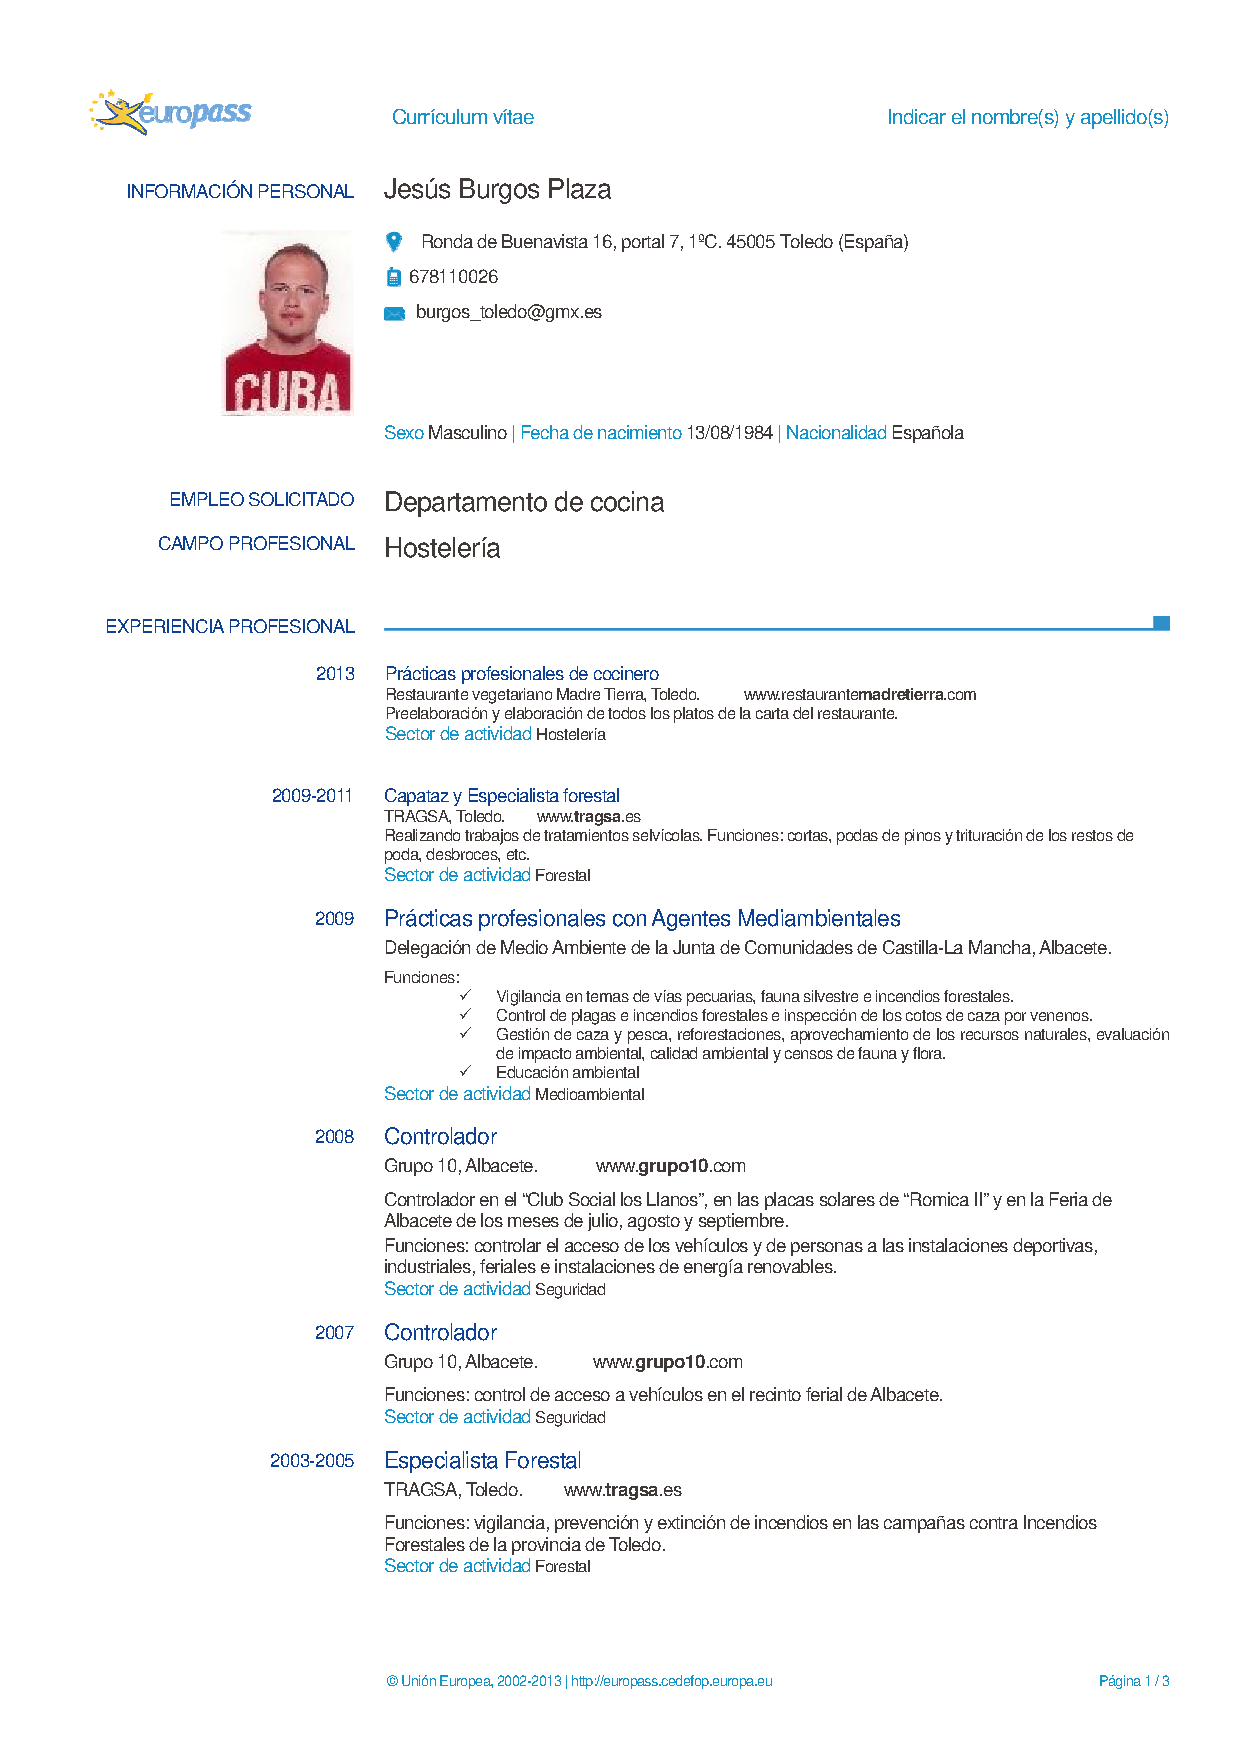
\includepdf[pages=-, width=1.3\textwidth, height=1.15\textheight, pagecommand={}]{CV.pdf}


\chapter{Instalaciones}
\label{chap:planos}

En el presente anexo se detallan los planos del centro de actividad y se muestran algunas fotos de las instalaciones.

\section{Restaurante \textbf{\textit{Quercus pyrenaica}}}
\label{chap:restaurante}

\begin{figure}[h!]
  \begin{center}
    \includegraphics[scale=0.75]{images/restaurante.jpg}
    \caption{Fachada del restaurante}
    \label{fig:restaurante}
  \end{center}
\end{figure}

El establecimiento se divide en las siguientes partes:

\subsection{Cocina}
\label{sec:restaurante:cocina}

\begin{figure}[h!]
  \begin{center}
    \includegraphics[scale=0.28]{images/cocina.jpg}
    \caption{Plano de la cocina}
    \label{fig:cocina}
  \end{center}
\end{figure}


\subsection{Sala}
\label{sec:restaurante:sala}

\begin{figure}[h]
  \begin{center}
    \includegraphics[scale=0.6]{images/sala.jpg}
    \caption{Plano de la sala}
    \label{fig:sala}
  \end{center}
\end{figure}


\subsection{Terraza}
\label{sec:restaurante:terraza}

\begin{figure}[h]
  \begin{center}
    \includegraphics[scale=0.6]{images/terraza.jpg}
    \caption{Plano de la terraza}
    \label{fig:terraza}
  \end{center}
\end{figure}

\newpage
\section{Bungalows}
\label{sec:bungalows}

\begin{figure}[h]
  \begin{center}
    \includegraphics[scale=0.9]{images/bungalows1.jpg}
    \caption{Imagen de los bungalows de capacidad para cuatro personas}
    \label{fig:bungalows1}
  \end{center}
\end{figure}

\begin{figure}[h]
  \begin{center}
    \includegraphics[scale=0.25]{images/bungalows2.jpg}
    \caption{Imagen de los bungalows de capacidad para dos personas}
    \label{fig:bungalows2}
  \end{center}
\end{figure}

\newpage
\section{Huerto ecológico para uso de cursos como abastecimiento de la cocina}
\label{sec:huerto}


\begin{figure}[h]
  \begin{center}
    \includegraphics[scale=0.28]{images/huertoEcologico.jpg}
    \caption{Fotografía del huerto ecológico}
    \label{fig:huertoEcologico}
  \end{center}
\end{figure}

\section{Invernadero subterráneo para productos agrícolas}
\label{sec:invSubterraneo}

\begin{figure}[h]
  \begin{center}
    \includegraphics[scale=0.7]{images/invernaderoSub.jpg}
    \caption{Fotografía del invernadero subterráneo}
    \label{fig:invernaderSub}
  \end{center}
\end{figure}


\newpage
\section{Invernadero reciclado para  cursos de jardinería}
\label{sec:invReciclado}

\begin{figure}[h]
  \begin{center}
    \includegraphics[scale=0.55]{images/invernaderRec.jpg}
    \caption{Fotografía del invernadero reciclado}
    \label{fig:invernaderRec}
  \end{center}
\end{figure}

\section{Huerto de  aromáticas}
\label{sec:aromaticas}

\begin{figure}[h]
  \begin{center}
    \includegraphics[scale=1]{images/huertoArom.jpg}
    \caption{Fotografía del huerto de aromáticas}
    \label{fig:huertoArom}
  \end{center}
\end{figure}

\newpage
\section{Aula de cursos formativos parte teórica y recepción}
\label{sec:aula}

En esta aula se encuentra, además, la recepción de la empresa.

\begin{figure}[h]
  \begin{center}
    \includegraphics[scale=0.6]{images/aula.jpg}
    \caption{Fotografía del aula de cursos formativos}
    \label{fig:aula}
  \end{center}
\end{figure}


 

\chapter{Puesta en marcha del complejo hostelero}
\label{chap:pasos}

Pasos seguidos y a seguir para la puesta en marcha del complejo hostelero:


\section{Cuenta atrás de un restaurante}
\label{sec:cuentaAtras}

\subsection{Fase conceptual}
\label{sec:conceptual}

18 meses -12 meses.

\begin{enumerate}
\item Estudio de mercado.
\item Análisis de las necesidades.
\item Definición del producto:
	\begin{enumerate}
		\item Nombre del complejo hostelero
		\item Concepto de la restauración
	\end{enumerate}
\item Elección del público-objetivo al que se quiere llegar.
\item Contacto con los arquitectos y financieros/discusión.
\item Anteproyecto.
\item Estudio financiero.
\item El proyecto se somete a las autoridades.
\item Proyecto de ejecución.
\item Contratación del director.
\item Metodología para la búsqueda de un precio máximo( precios de venta de las prestaciones de la competencia )
\item Programa general de ventas ( carta de platos, precios de cursos, precios de bungalows, fichas técnicas, etc.)
\item Autorizaciones administrativas.
\end{enumerate}

\subsection{Fase de Organización I}
\label{sec:organizacion1}

12 meses - 6 meses

\begin{enumerate}
\item Equipamiento del complejo hostelero ( cocina, vestuario, oficina, bungalows, etc.)
	\begin{enumerate}
	\item Maquinarias.
	\item Mobiliario.
	\end{enumerate}
\item Adquisición de la ropa blanca y uniformes, pequeño inventario ( vasos, cubiertos, vajilla, material de oficina)
\item Organigrama/ cálculo de la plantilla/pliego de condiciones.
\item Definición del modo de explotación / días-horas de apertura, etc.
\item Presupuesto de explotación/ implantación de la contabilidad.
\item Dossiers de seguros y contratos de mantenimiento.
\item Impresión de los documentos administrativos.
\item Programa de contratación de los directivos ( chefs de cocina, jefes de servicio)
\item Objetivos de marketing y elección de una estrategia de comercialización.
\end{enumerate}

\subsection{Fase de Organización II}
\label{sec:organizacion2}

6 meses - 3 meses

\begin{enumerate}
\item Preparación del reglamento interno.
\item Preparación del plan de empresa.
\item Solucionar las cuestiones relativas al lavado de mantelería como de uniformes.
\item Plan de utilización de los espacios frigoríficos, reservas, etc.
\item Adquisición de los accesorios del restaurante.
\item Elección de una música de ambiente para el restaurante.
\item Control y corrección de las fichas técnicas con el chef de cocina.
\item Impresión de cartas, menús y cartas de bebidas.
\item Rótulos/ señalización interna.
\item Definición de una política medioambiental.
\end{enumerate}

\subsection{Fase de Lanzamiento}
\label{sec:lanzamiento}

3 meses -1 mes

\begin{enumerate}
\item Negociaciones con los proveedores/ elección y lista de proveedores de mercancías no perecederas y perecederas.
\item Definición de una animación de apertura.
\item Plan de comercialización para los3 meses siguientes a la apertura ( publicidad externa, merchandising interno)
\item Reserva de personal extra para la inauguración.
\item Contratación del personal. Contratación prevista para 10-15 días antes de la inauguración según los puestos de trabajo.
\item Envío por correo de las invitaciones para la inauguración.
\end{enumerate}

\subsection{Fase previa a la apertura}
\label{sec:previa}
1 mes - 10 días

\begin{enumerate}
\item Control de los puntos nos resueltos y toma de decisiones en consecuencia.
\item Petición y recepción de las mercancías no perecederas.
\item Ensayo general de todo el equipamiento con los jefes de servicio incluyendo la iluminación de emergencias, los apartados de seguridad.
\item Primera limpieza general.
\item Adjudicación y aceptación nominativas de equipamientos específicos.
\item Fijación de los precios de venta definitivos ( últimas correcciones eventuales para los platos del día cuyos precios no están impresos en las cartas)
\item Distribución de los uniformes.
\item Información a la política de cara a la inauguración.
\end{enumerate}

\subsection{Fase de Apertura}
\label{sec:apertura}

Días atrás

\begin{itemize}[label={}]
\item \textbf{X-10} Curso para todos los mandos.
\item \textbf{X-9} Curso para todo los mandos. Formación específica para los empleados ( utilización de los equipamientos, máquinas, informática, etc.).
\item \textbf{X-8} Curso de seguridad ( vandalismo, fuego, robo, accidentes)
\item \textbf{X-7} Cursos de previsión de ventas
\item \textbf{X-6} Día libre
\item \textbf{X-5} Limpieza y arreglo ( poner orden)
\item \textbf{X-4} Instrucciones sobre la inauguración oficial o apertura.
\item \textbf{X-3} Preparación de los platos de la carta. Degustación. Críticas.
\item \textbf{X-2} Puesta a punto de todos los departamentos.
\item \textbf{X-1} Puesta a punto de todos los dptos., decoración floral, dossier de prensa. Media jornada de descanso.
\item \textbf{X}   Inauguración oficial.
\item \textbf{X+1} Limpieza general. Análisis de los puntos débiles eventuales en la jornada oficial. Correcciones inmediatas si fuera necesario. Adoptar un ritmo normal de trabajo. Planificación de los platos del día. Planificación de reuniones de trabajo por sector o reuniones de mejora. Agradecimientos de la dirección a los invitados y a los empleados)
\item \textbf{X+10} Control de la formación del personal. Primer chequeo de la empresa.
\end{itemize}

\section{Horarios}
\label{sec:horarios}

\begin{figure}[h]
  \begin{center}
    \includegraphics[scale=0.5]{images/horarios.jpg}
    \caption{Horarios de atención al público}
    \label{fig:horarios}
  \end{center}
\end{figure}

\section{Fecha de los cursos}
\label{sec:cursos}

Los cursos ofrecidos por la empresa se realizaran en temporada baja, según aparece en el calendario.
Realizándose de principalmente los fines de semana:

\begin{itemize}
\item de 8:00 h a 11:00  cursos forestales
\item de 18:00 h a 21:00 cursos de cocina
\end{itemize}

\emph{Nota}: los cursos solo se realizarán bajo acuerdo previo telefónicamente.

En la Figura \ref{fig:cursos} se muestra el calendario de cursos previsto para el año 2014.

\begin{figure}[ht]
  \begin{center}
    \includegraphics[scale=0.6]{images/cursos.jpg}
    \caption{Calendario de cursos en las instalaciones}
    \label{fig:cursos}
  \end{center}
\end{figure}

\newpage
\section{A qué nos queremos parecer}
\label{sec:parecer}

El objetivo es conseguir unas instalaciones de muy alta calidad, con un excelente diseño y alto grado de funcionalidad para los empleados y comodidad para los clientes.

\begin{figure}[h]
  \begin{center}
    \includegraphics[scale=0.4]{images/parecer1.jpg}
    \caption{Fotografía detalle de la sala}
    \label{fig:parecer1}
  \end{center}
\end{figure}

\begin{figure}[ht]
  \begin{center}
    \includegraphics[scale=0.4]{images/parecer2.jpg}
    \caption{Fotografía del interior de la cocina}
    \label{fig:parecer2}
  \end{center}
\end{figure}

\chapter{Recetas del restaurante}
\label{chap:recetas}

\section{Falafel con lechuga de la huerta}
\label{sec:falafel}

Se dejan los garbanzos en remojo el día anterior con agua tibia. Posteriormente se trituran hasta obtener una pasta a la cual se le incorpora la cebolla en brunoixe, el ajo en brunoixe, el impulsor, la harina, la  sal, el perejil y el comino molido. Se mezcla bien y se moldea.

Se fríen hasta que estén bien dorados.

\begin{figure}[h]
  \begin{center}
    \includegraphics[scale=0.13]{images/falafel.jpg}
    \caption{Falafel con lechuga de la huerta}
    \label{fig:falafel}
  \end{center}
\end{figure}

\section{Degustación de \emph{Patés vegetarianos}}
\label{sec:pates}

\subsection{Paté de champiñón}
\label{sec:patechampi}
\begin{itemize}
\item Picamos tanto el ajo con la cebolla
\item Doramos los ajos en aceite y luego la cebolla, hasta que esté bien pochada.
\item Añadimos al sofrito el boletus cortado en láminas y dejamos que se hagan con los otros dos ingredientes
\item Ponemos a punto de sal
\item Trituramos en la termomix hasta que nos queda una masa resultante parecida a un paté.
\end{itemize}

\subsection{Paté de berenjena}
\label{sec:pateberen}
\begin{itemize}
\item Picamos tanto el ajo con la cebolla
\item Doramos los ajos en aceite y luego la cebolla, hasta que esté bien pochada.
\item Añadimos al sofrito la berenjena troceado y dejamos que se hagan con los otros dos ingredientes
\item Ponemos a punto de sal
\item Trituramos en la termomix hasta que nos quede una masa resultante parecida a un paté.
\end{itemize}

\subsection{Humus}
\label{sec:humus}
\begin{itemize}
\item En un bol añadimos los ingredientes: garbanzos, tahini, ajo, comino, pimentón, perejil, aceite de oliva, perejil, sal y el zumo de limón. etc. A todo ello, incorporamos un poco de agua. Trituramos todos los ingredientes en la termomix.
\end{itemize}

\section{Ensalada \emph{Quercus}}
\label{sec:ensaladaQ}

\begin{figure}[h]
  \begin{center}
    \includegraphics[scale=0.12]{images/ensaladaQuercus.jpg}
    \caption{Ensalada \emph{Quercus}}
    \label{fig:ensaladaQuercus}
  \end{center}
\end{figure}

Ingredientes:
\begin{itemize}
\item Lechuga mezclum
\item Queso de cabra
\item Membrillo
\item Granada
\item Champiñón laminado
\item Aceite de oliva
\item Vinagre de Módena
\item Sal
\end{itemize}
Elaboración:
\begin{itemize}
\item Mezclar todo y aliñar con el aceite, vinagre y sal
\end{itemize}

\section{Témpura de verduras}
\label{sec:tempura}

\begin{figure}[h]
  \begin{center}
    \includegraphics[scale=0.2]{images/tempura.jpg}
    \caption{Témpura de verduras}
    \label{fig:tempura}
  \end{center}
\end{figure}

Ingredientes:
\begin{itemize}
\item Pimiento rojo en tiras
\item Pimiento verde en tiras
\item Cebolla en aros
\item Zanahoria en bastones
\item Champiñón laminado
\item Berenjena cortada a la española
\item Calabacín en rodajas.
\item Cerveza muy fría
\item Harina de trigo
\item Sal
\end{itemize}

Elaboración:
\begin{itemize}
\item Freír todos los ingredientes en la pasta resultante de mezclar la harina con la cerveza y una pizca de sal.
\end{itemize}

\section{Parrillada de verduras}
\label{sec:parrillada}

\begin{figure}[h]
  \begin{center}
    \includegraphics[scale=0.3]{images/parrillada.jpg}
    \caption{Parrillada de verduras}
    \label{fig:parrillada}
  \end{center}
\end{figure}

Ingredientes:
\begin{itemize}
\item Cebolla en rodajas.
\item Pimiento verde en tiras
\item Pimiento rojo en tiras
\item Berenjena en rodajas
\item Calabacín en rodajas
\item Champiñón en rodajas
\item Sal
\item Aceite de oliva
\end{itemize}

Elaboración:
\begin{itemize}
\item Colocar los ingredientes encima de una parrilla caliente previamente engrasada hasta que estén bien doradas las marcas de la parrilla por ambos lados.
\end{itemize}

\section{Primeros Platos}
\label{sec:primeros}

\subsection{Falsos escalopines de tofu al pesto}
\label{sec:escalopines}

Hacemos un pesto con piñones, el queso, el aceite y la albahaca.
Gran parte de ese pesto lo mezclamos con el tofu fresco escurrido y con la harina. Damos forma y enharinamos. Freír y emplatar con salsa de pesto.

\subsection{Risotto de setas de temporada y espárragos trigueros}
\label{sec:risotto}

Rehogamos con aceite el ajo, el puerro, la cebolla, los pimientos, la zanahoria, las setas y los espárragos. Añadimos el arroz y echamos el caldo de verduras poco a poco según vaya necesitando el arroz. Cuando este prácticamente al punto añadimos el queso rallado. Mezclamos bien y emplatamos.

\begin{figure}[h]
  \begin{center}
    \includegraphics[scale=0.07]{images/risotto.jpg}
    \caption{Risotto de setas de temporada y espárragos trigueros}
    \label{fig:risotto}
  \end{center}
\end{figure}

\subsection{Patatas revolconas de seitán}
\label{sec:revolconas}

\begin{figure}[h]
  \begin{center}
    \includegraphics[scale=0.7]{images/revolconas.jpg}
    \caption{Patatas revolconas de seitán}
    \label{fig:revolconas}
  \end{center}
\end{figure}

Cocemos las patatas con la cebolla. Retiramos la cebolla y hacemos un puré.
Por otro lado adobamos el seitán en trozos pequeños, los freímos con el adobo y el aceite y los retiramos. Echamos el puré de patatas y mezclamos bien. Emplatamos con algunos trozos de seitán entre el puré y unos pocos por encima.

\newpage
\subsection{Revuelto de setas de temporada}
\label{sec:revueltoTemporada}

Se hace un sofrito con el ajo picado y la cebolla, añadimos las setas y rehogamos. Echamos el huevo batido  y removemos, retirando del fuego si es preciso hasta que tengamos una textura melosa.

\begin{figure}[h]
  \begin{center}
    \includegraphics[scale=0.25]{images/revueltoTemporada.jpg}
    \caption{Revuelto de setas de temporada}
    \label{fig:revueltoTemporada}
  \end{center}
\end{figure}


\subsection{Huevo roto sobre soja texturizada adobada}
\label{sec:huevo}
\begin{itemize}
\item Hidratamos la soja texturizada, escurrimos y adobamos.
\item Freímos y ponemos un huevo mollet para que el camarero  lo corte al cliente
\end{itemize}

\section{Segundos Platos}
\label{sec:segundos}

\subsection{Falso cordón blue de seitán con salsa de piquillo}
\label{sec:cordon}

Cortamos el seitán en filetes de medio centímetro de grosor. Untamos el pate en una de las caras de los filetes y metemos una loncha de queso entre medias de las dos caras con paté. Lo empanamos con el pan rallado y los kikos. 
Para la salsa sofreímos el ajo picado y la cebolla. Añadimos el pimiento de piquillo cortado y rehogamos. Añadimos la nata y trituramos. Si resulta muy espesa pasamos por un chino.

\begin{figure}[h]
  \begin{center}
    \includegraphics[scale=0.4]{images/cordonBlue.jpg}
    \caption{Falso cordón blue de seitán con salsa de piquillo}
    \label{fig:cordonBlue}
  \end{center}
\end{figure}

\subsection{Hamburguesa de lentejas con arroz}
\label{sec:hamburguesa}

\begin{figure}[h]
  \begin{center}
    \includegraphics[scale=0.4]{images/hamburguesa.jpg}
    \caption{Hamburguesa de lentejas con arroz}
    \label{fig:hamburguesa}
  \end{center}
\end{figure}

\begin{itemize}
\item Se cubren las lentejas con agua y se cuecen a fuego lento hasta que estén blandas,
\item Se escurren y se pasan por la batidora o el pasapurés.
\item Se mezcla con las lentejas y el resto de los Ingredientes.
\item Se deja reposar todo el tiempo que se pueda para que se seque un poco la masa.
\item Se forman las hamburguesas, se ponen en una bandeja de horno engrasada y se asan en el gratinador del horno primero por un lado y luego por el otro.
\end{itemize}



\subsection{Hamburguesa de zanahoria}
\label{sec:hamburZana}

Se hace un sofrito de ajo, con la cebolla y la zanahoria. Añadimos la soja texturizada hidratada previamente y rehogamos. Añadimos harina hasta obtener una masa. Moldeamos y hacemos al horno o a la plancha. 

\begin{figure}[h]
  \begin{center}
    \includegraphics[scale=0.25]{images/hamburguesaZana.jpg}
    \caption{Hamburguesa de zanahoria}
    \label{fig:hamburguesaZana}
  \end{center}
\end{figure}

\subsection{Falso escalope de seitán a la mostaza con nido de patata paja y huevo mollet}
\label{sec:escalopeSeitan}

Para los escalopes mezclamos el gluten con todos los ingredientes hasta obtener una masa homogénea. La enrollamos con film para darle forma y lo pinchamos, para posteriormente cocerlo a fuego lento. Una  vez hecho esto, dejamos enfriar y cortamos escalopes de esta pieza de  seitán. Marcamos a la plancha.
Por otro lado cortamos las patatas en patata paja y las freímos con forma de nido. Dentro del cual ponemos un huevo mollet.

\subsection{Mousaka}
\label{sec:musaka}
\begin{itemize}
\item Se parte la cebolla fina y se rehoga en el aceite. Se añade el ajo
\item Machacado, los champiñones en láminas, los tomates pelados y cortados,
\item La soja texturizada, el caldo y el perejil y se cuece a fuego lento unos 20 minutos.
\item Se parte la berenjena en láminas finas a lo largo y se cuece al vapor.
\item En una fuente de horno untada de aceite se pone una capa de berenjenas, a continuación se cubre con una capa de la salsa. Se van poniendo capas hasta terminar con una de berenjenas. Se pone el queso rallado por encima.
\item Se baten los huevos, se mezclan con el yogurt y se pone esta mezcla por encima de las berenjenas.
\item Se mete en el horno a 1 80~ unos 30 minutos, hasta que esté dorado.
\end{itemize}

\begin{figure}[h]
  \begin{center}
    \includegraphics[scale=0.7]{images/musaka.jpg}
    \caption{Musaka}
    \label{fig:musaka}
  \end{center}
\end{figure}

\subsection{Canelones de berenjena soja con pastel de patatas}
\label{sec:canelones}
\begin{itemize}
\item Cortamos las berenjenas en lonchas muy finas con la corta fiambres y marcamos a la plancha.
\item Para el relleno hidratamos soja texturizada. Realizamos una salsa de tomate e incorporamos la soja. Dejamos cocer con la salsa. \item \item Albardamos esta farsa con las láminas de berenjenas.
\item Para el pastel cortamos las patatas en rodajas, añadimos la nata junto con los huevos batidos (previamente mezclado) junto con la sal. 
\item Horneamos hasta que el pastel esté cuajado.
\end{itemize}

\begin{figure}[h]
  \begin{center}
    \includegraphics[scale=0.2]{images/canelones.jpg}
    \caption{Canelones de berenjena soja con pastel de patatas}
    \label{fig:canelones}
  \end{center}
\end{figure}

\subsection{Lasaña de setas}
\label{sec:lasana}
\begin{itemize}
\item Por un lado cocemos las pastas de lasaña.
\item Por otro hacemos un sofrito de ajo y cebolla al que añadimos las setas y las rehogamos. 
\item Por otro hacemos una roux con el aceite de oliva y de harina tpt. Añadimos la leche caliente y varillamos hasta conseguir una bechamel sin grumos.
\item Ponemos 2 capas intercaladas de pasta y el sofrito con las setas, empezando y terminando con una de pasta y echamos la bechamel.
\end{itemize}

\begin{figure}[h]
  \begin{center}
    \includegraphics[scale=0.5]{images/lasana.jpg}
    \caption{Lasaña de setas}
    \label{fig:lasana}
  \end{center}
\end{figure}

\section{Postres}
\label{sec:postres}

\subsection{Batido de frutos del bosque}
\label{sec:batido}

Trituramos los frutos, mezclamos con el azúcar y la leche hasta que el líquido resultante quede homogéneo.

\begin{figure}[h]
  \begin{center}
    \includegraphics[scale=0.3]{images/batidoBosque.jpg}
    \caption{Batido de frutos del bosque}
    \label{fig:batidoBosque}
  \end{center}
\end{figure}

\subsection{Batido de uvas}
\label{sec:batidoUva}
Trituramos las uvas, mezclamos con el azúcar y la leche hasta que el líquido resultante quede homogéneo.

\begin{figure}[h]
  \begin{center}
    \includegraphics[scale=0.5]{images/batidoUva.jpg}
    \caption{Batido de uvas}
    \label{fig:batidoUva}
  \end{center}
\end{figure}

\subsection{Helado de uva}
\label{sec:heladoUva}

Hacemos una crema inglesa con las yemas, el azúcar y la leche. Añadimos la nata y el zumo de uva. Mezclamos todo bien y metemos en la heladera hasta que tenga la consistencia deseada.

\begin{figure}[h]
  \begin{center}
    \includegraphics[scale=0.3]{images/heladoUva.jpg}
    \caption{Helado de uva}
    \label{fig:heladoUva}
  \end{center}
\end{figure}

\subsection{Tiramisú}
\label{sec:tiramisu}

Para el bizcocho plancha:

\begin{itemize}
\item Batimos los huevos con el azúcar. Se añade la harina, el impulsor y 0,250  ml de agua templada. Emulsionamos y metemos en una manga pastelera. 
\item Extendemos en una bandeja para el horno. 
\item Horneamos a 215º durante 8 min.
\end{itemize}
Para el tiramisú:
\begin{itemize}
\item Echar la mitad del azúcar en la nata líquida y montarla hasta que quede muy compacta (debe estar fría y a ser posible en un recipiente metálico frío).
\item Separar las claras y las yemas de los huevos.
\item Montar las claras a punto de nieve (mejor si se echan unas gotas de limón o vinagre).
\item Mezclar despacio con un cucharón el queso mascarpone y las yemas de huevo, añadiendo el resto del azúcar (no utilizar la batidora).
\item Cuando el queso y las yemas estén mezclados juntar con la nata montada y las claras a punto de nieve y mezclar todo bien, pero despacio.
\item En el café caliente disolver un tercio del chocolate en polvo y echar un chorrito del..licor.
\item Mojar muy ligeramente los bizcochos en el café sin dejar que se empapen y disponer la mitad de ellos cubriendo el fondo de una fuente.
\item Echar la mitad de la mezcla sobre los bizcochos cubriéndolos uniformemente.
\item Poner una nueva capa de bizcochos mojados ligeramente sobre la mezcla.
\item Echar el resto de la mezcla sobre la segunda capa de bizcochos
\item Espolvorear bien el chocolate en polvo sobre la mezcla
\item Dejar reposar al menos 6 horas (preferible 24 horas)
\end{itemize}

\begin{figure}[h]
  \begin{center}
    \includegraphics[scale=0.25]{images/tiramisu.jpg}
    \caption{Tiramisú}
    \label{fig:tiramisu}
  \end{center}
\end{figure}

\subsection{Brownie con helado de vainilla}
\label{sec:brownieVa}

Mezclamos la harina, con la mantequilla, con la cobertura de chocolate, con los huevos, el azúcar y las nueces. Lo metemos al horno durante unos 35 min. aprox. A 180ºC el cual hemos precalentado previamente.

\begin{figure}[h]
  \begin{center}
    \includegraphics[scale=0.8]{images/brownie.jpg}
    \caption{Brownie con helado de vainilla}
    \label{fig:brownie}
  \end{center}
\end{figure}


\chapter{Gestión y Valoración de Platos}
\label{chap:valPlatos}

En las siguientes páginas se muestran las distintas tablas creadas para obtener la valoración real de cada uno de los platos ofertados en el restaurante.

\section{Para empezar}
\label{sec:valCarta}

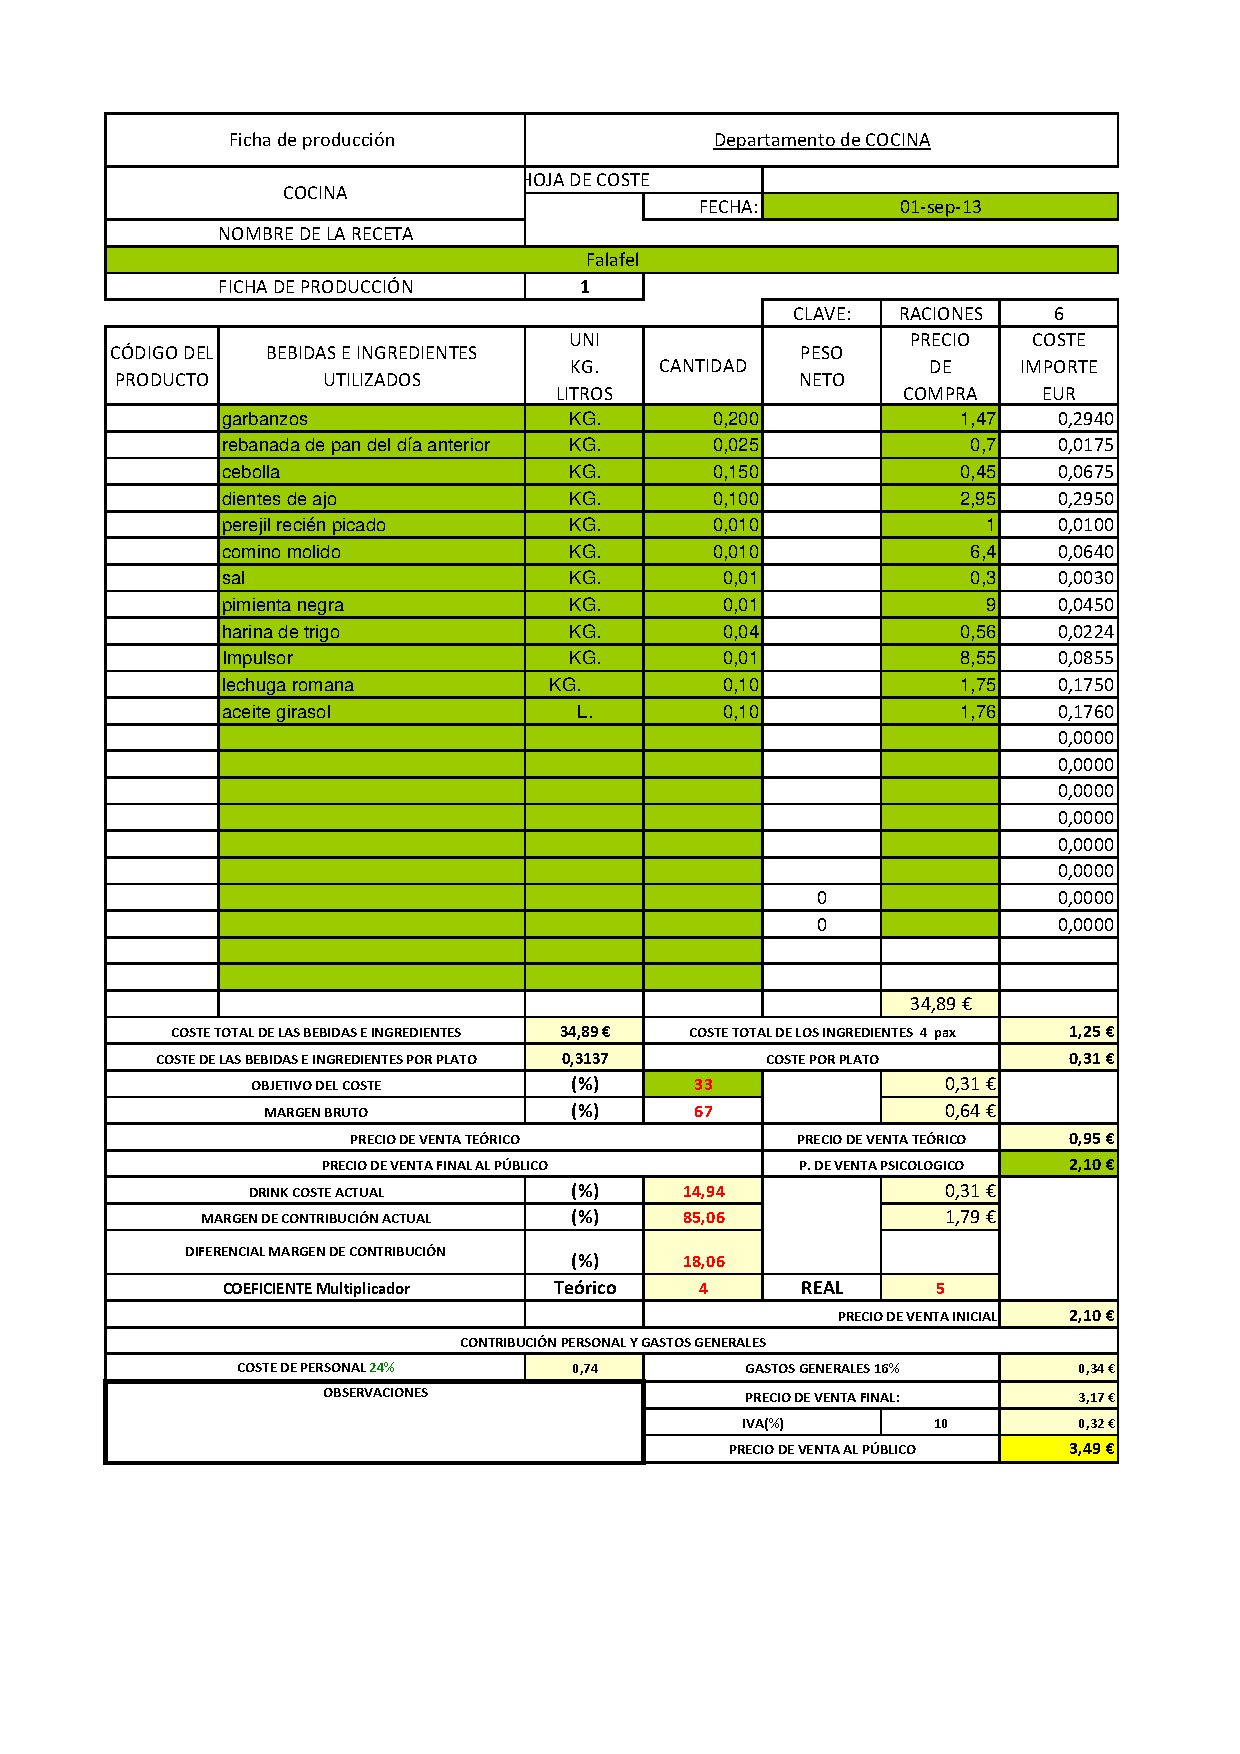
\includepdf[pages=-, width=1.1\textwidth, height=1.1\textheight, pagecommand={}]{tablas/Falafel.pdf}
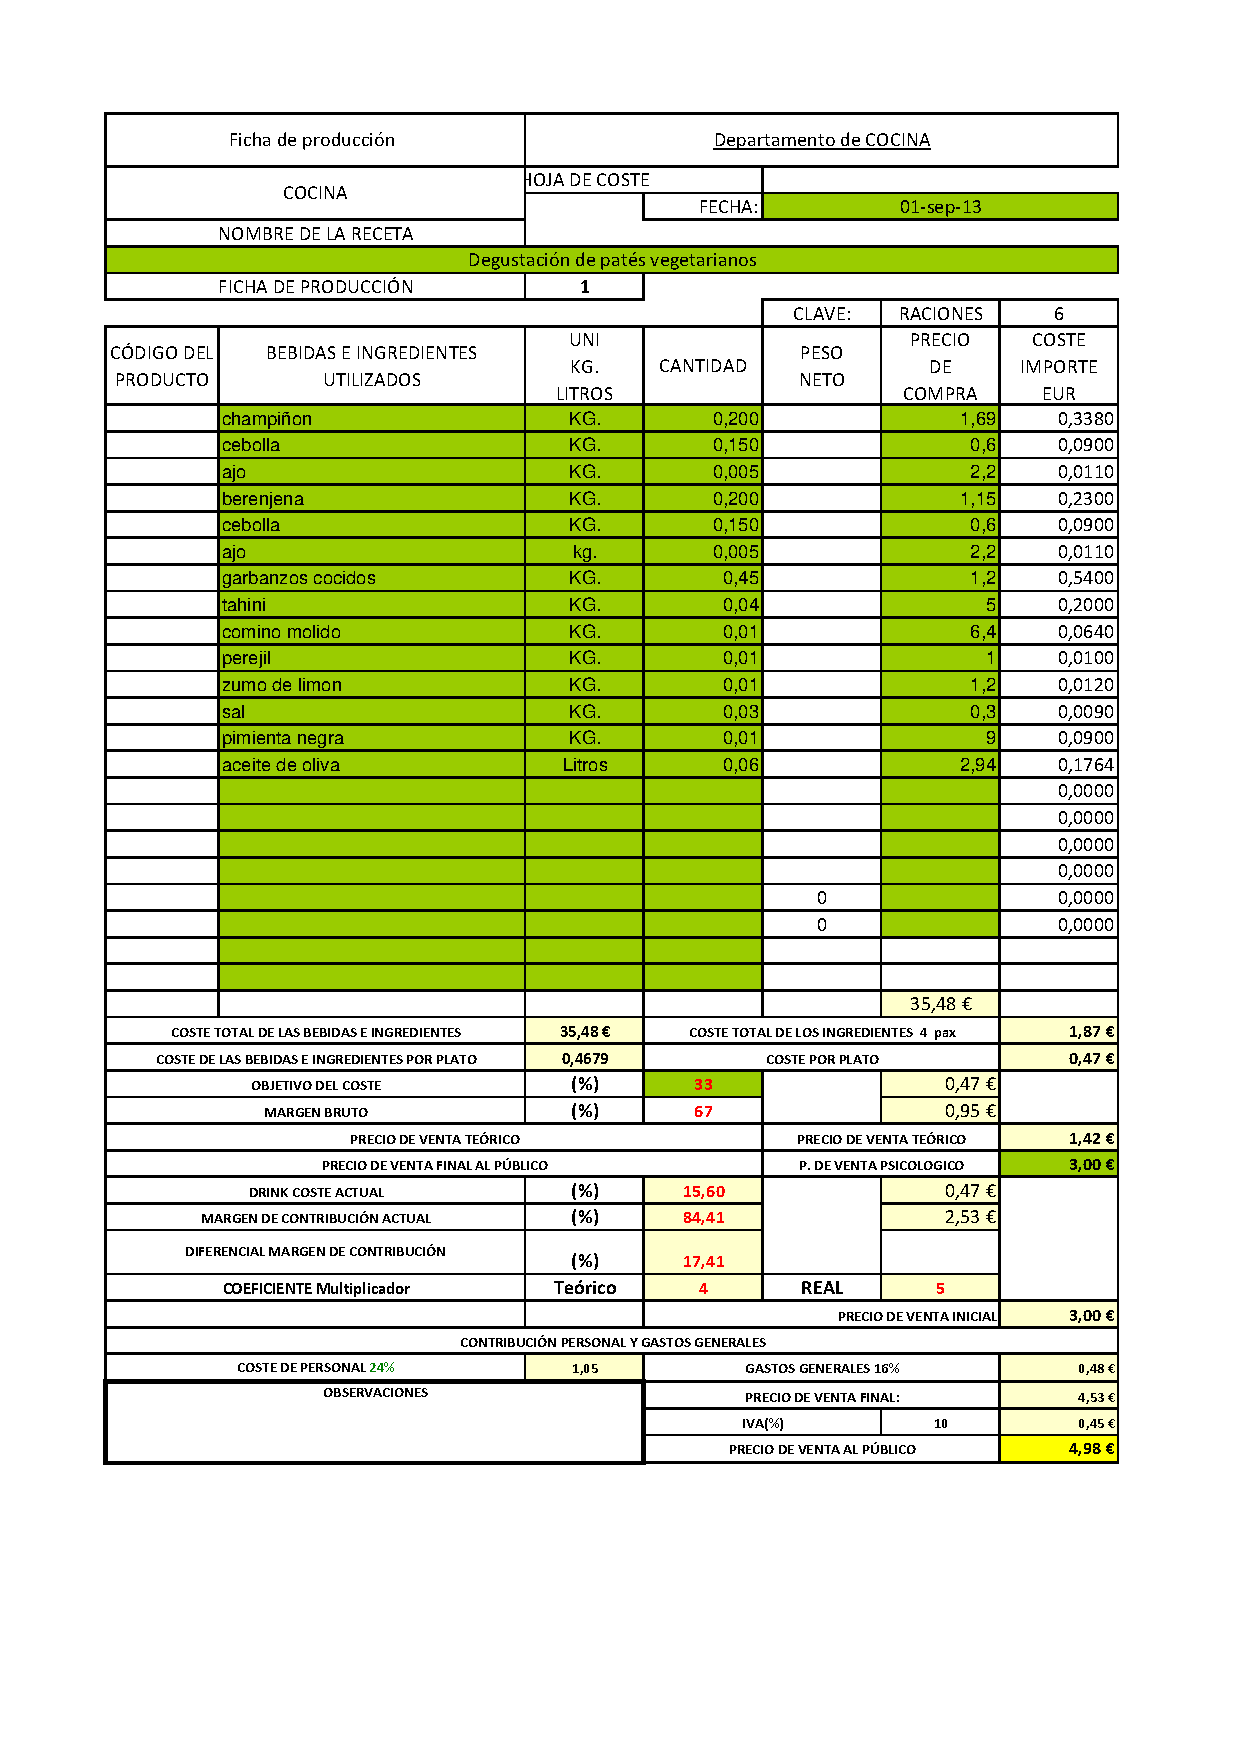
\includepdf[pages=-, width=1.1\textwidth, height=1.1\textheight, pagecommand={}]{tablas/Pates.pdf}
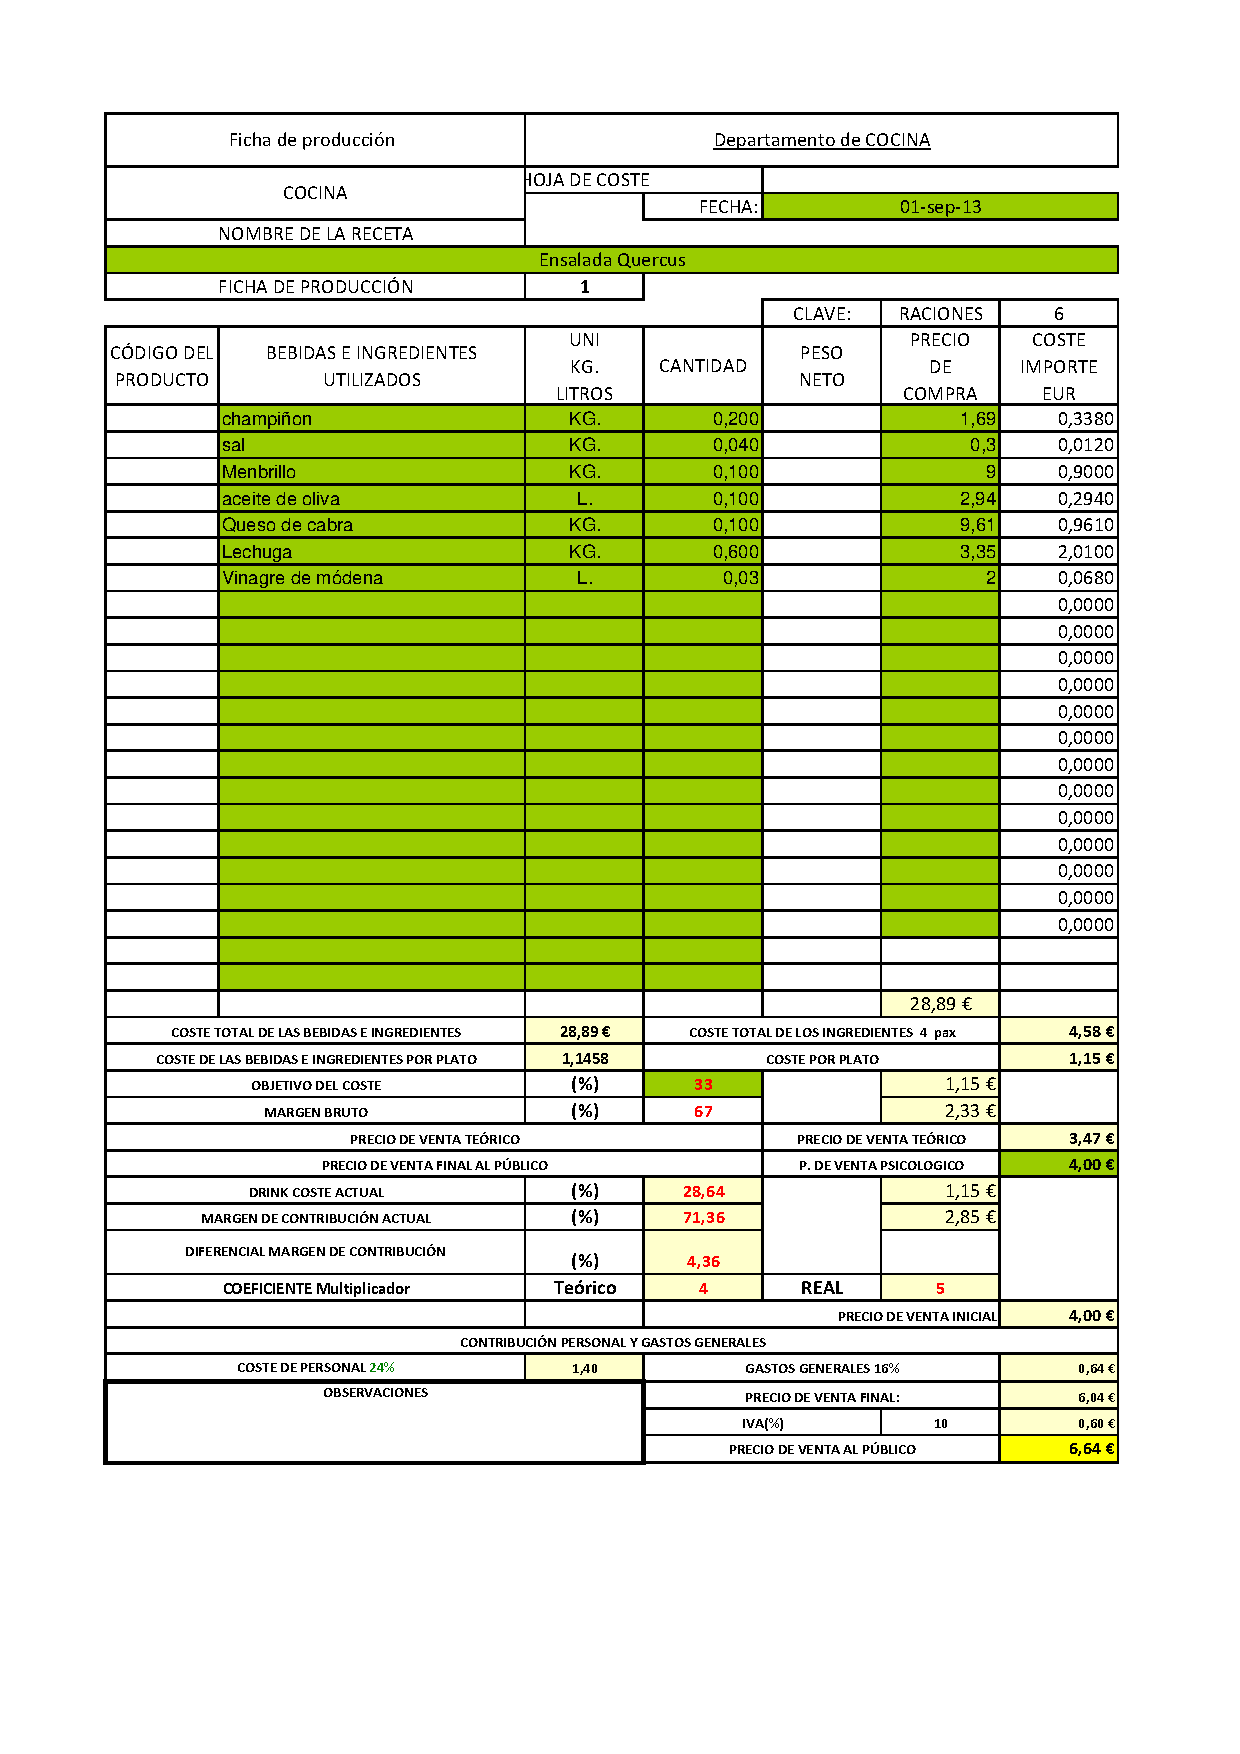
\includepdf[pages=-, width=1.1\textwidth, height=1.1\textheight, pagecommand={}]{tablas/EnsaladaQuercus.pdf}
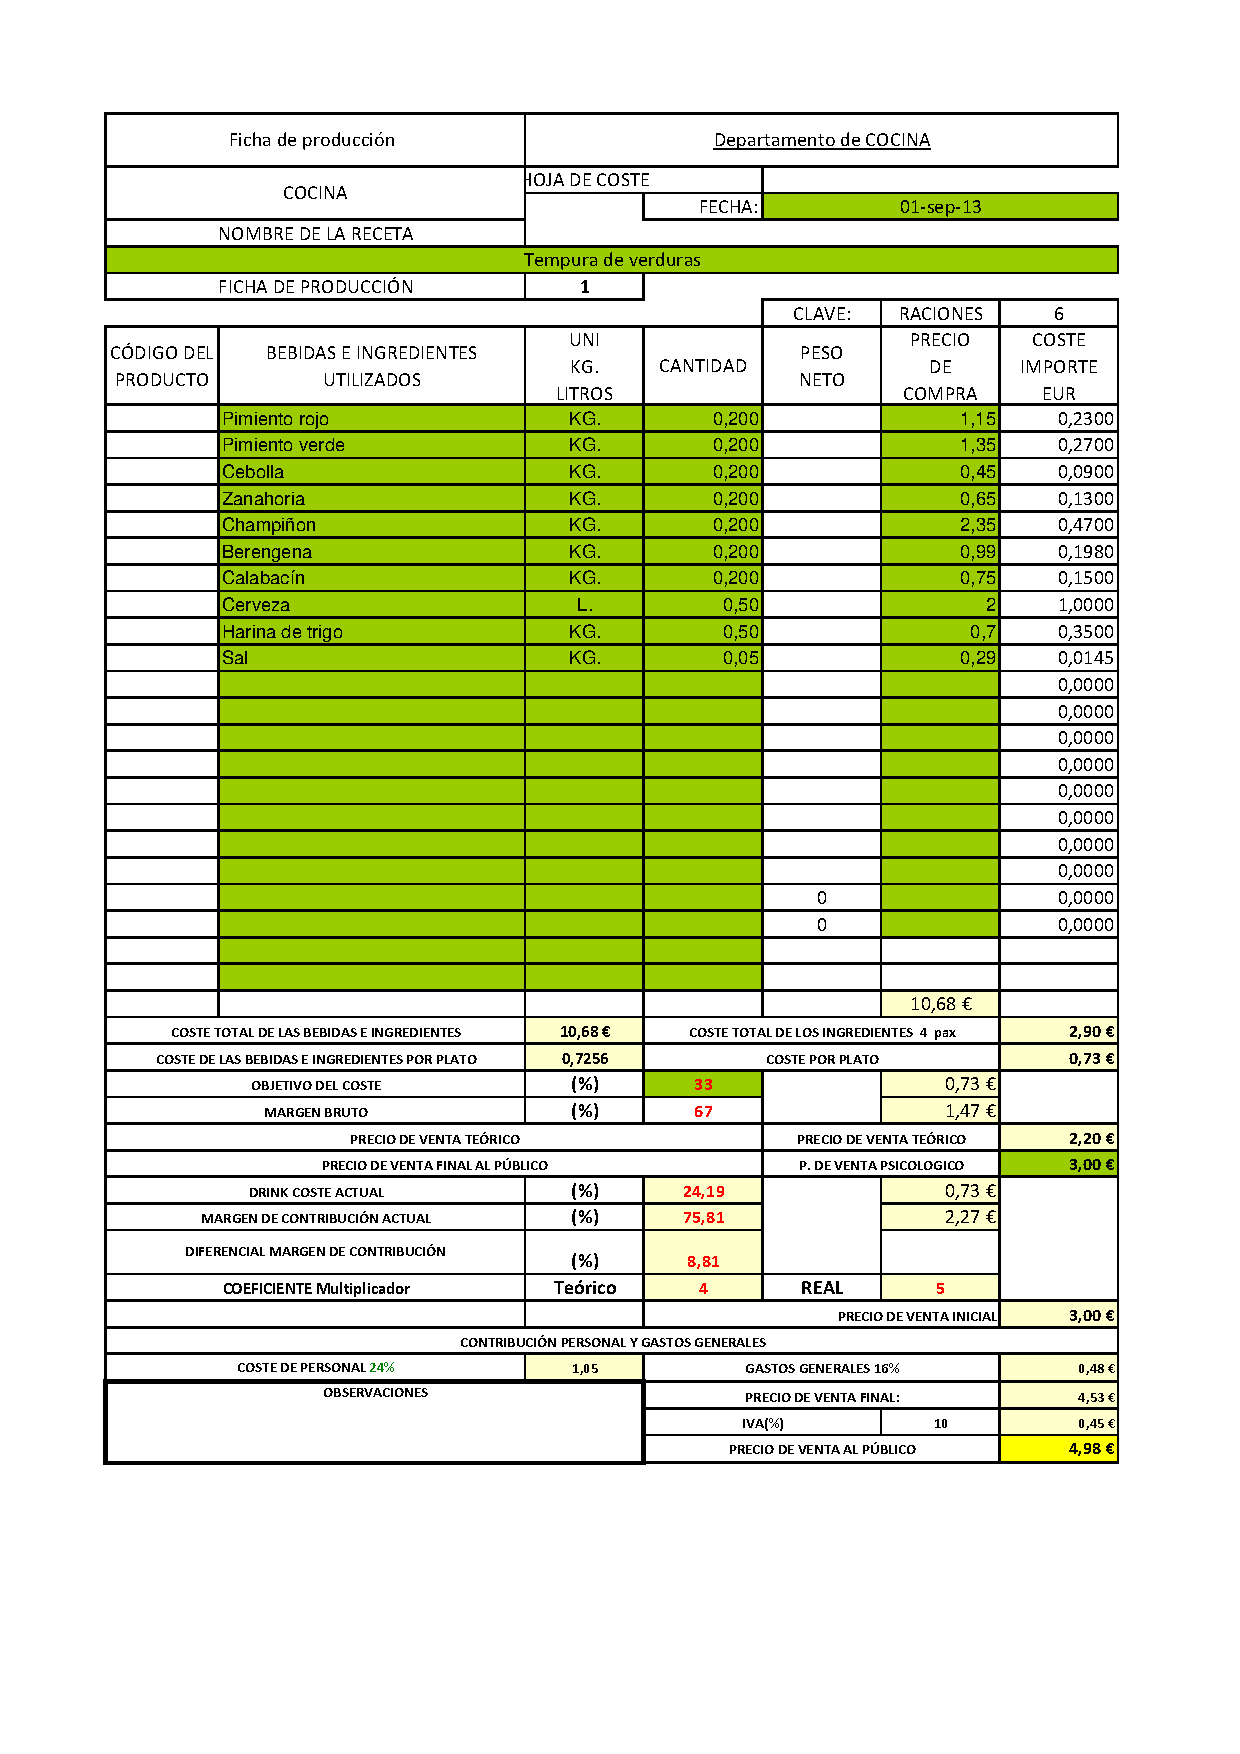
\includepdf[pages=-, width=1.1\textwidth, height=1.1\textheight, pagecommand={}]{tablas/Tempura.pdf}
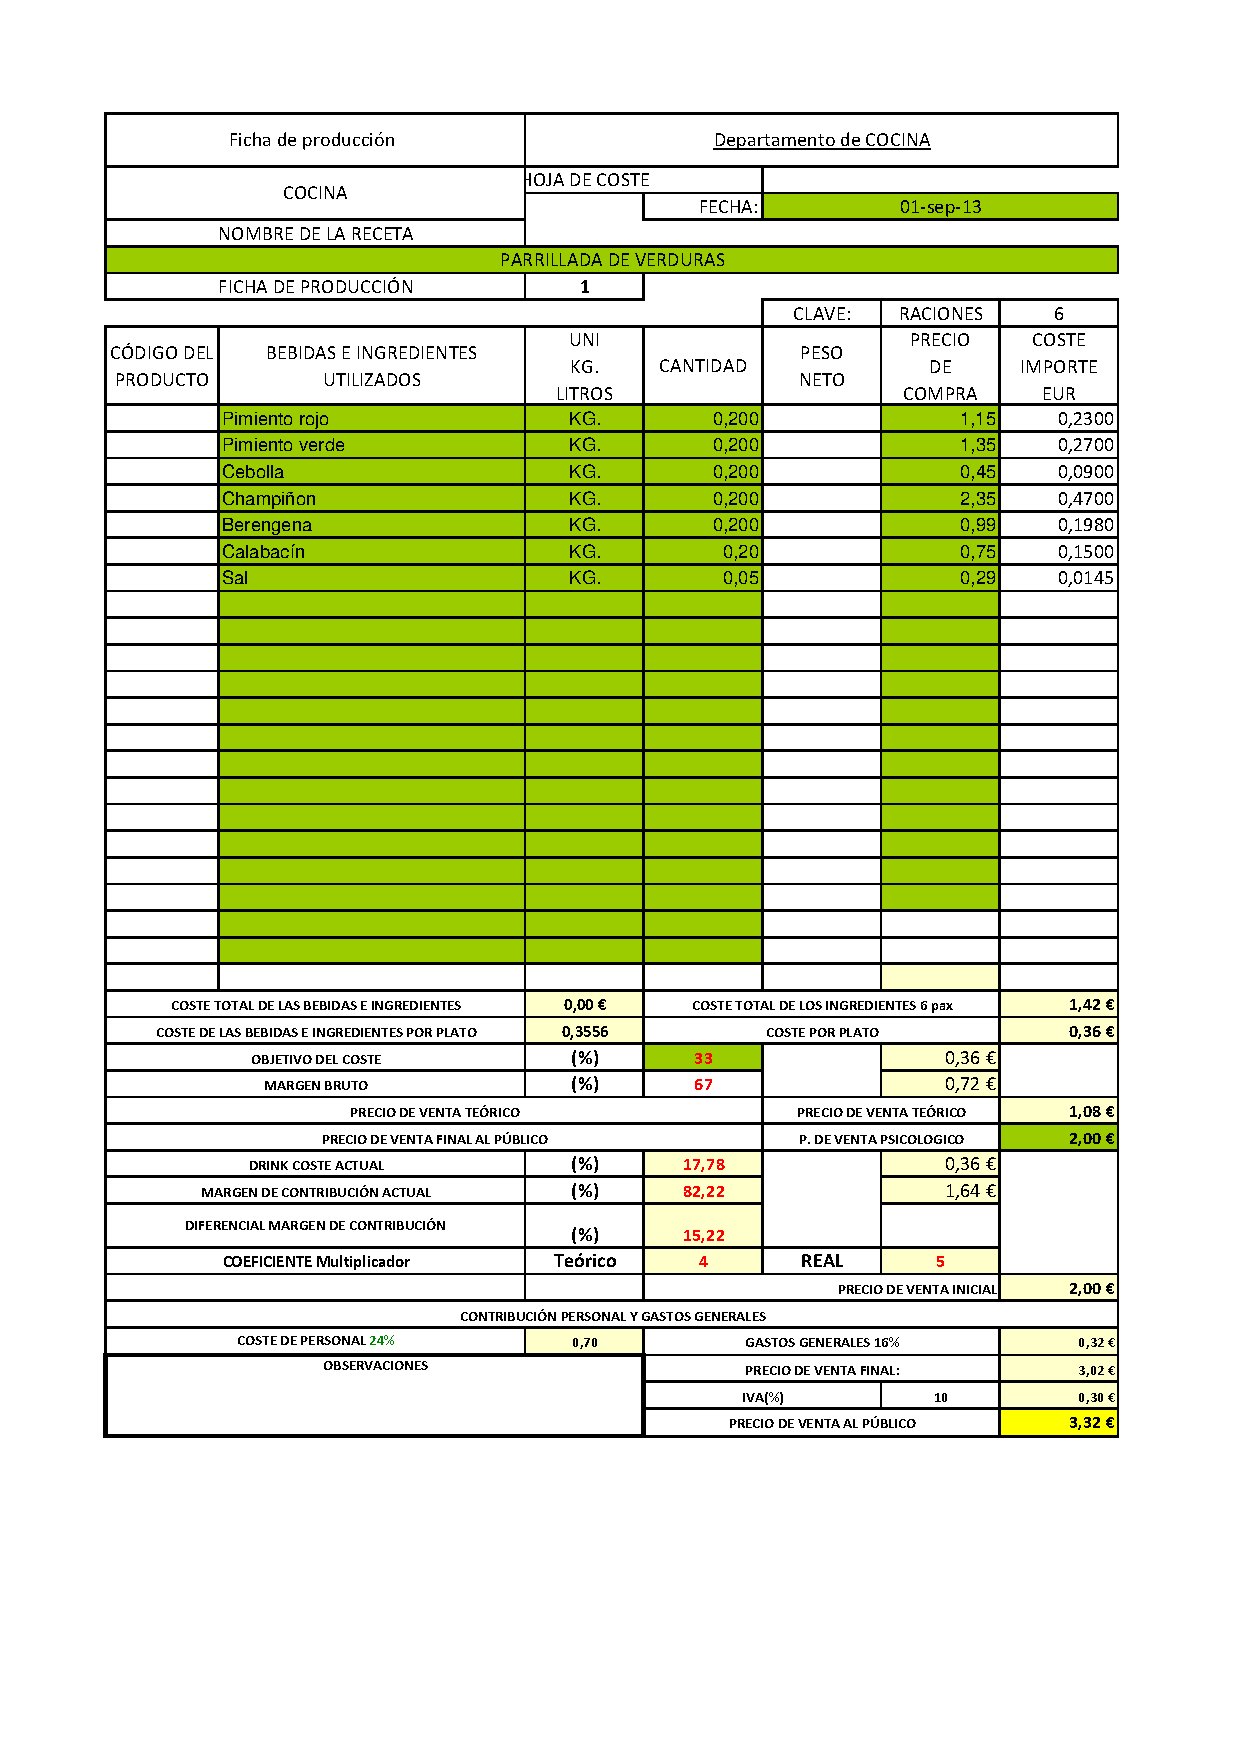
\includepdf[pages=-, width=1.1\textwidth, height=1.1\textheight, pagecommand={}]{tablas/Parrillada.pdf}

\section{Primeros Platos}
\label{sec:valPrimeros}

\includepdf[pages=-, width=1.1\textwidth, height=1.1\textheight, pagecommand={}]{tablas/primeros/FalsoEscalopin.pdf}
\includepdf[pages=-, width=1.1\textwidth, height=1.1\textheight, pagecommand={}]{tablas/primeros/Risotto.pdf}
\includepdf[pages=-, width=1.1\textwidth, height=1.1\textheight, pagecommand={}]{tablas/primeros/Revolconas.pdf}
\includepdf[pages=-, width=1.1\textwidth, height=1.1\textheight, pagecommand={}]{tablas/primeros/Revuelto.pdf}
\includepdf[pages=-, width=1.1\textwidth, height=1.1\textheight, pagecommand={}]{tablas/primeros/huevoRoto.pdf}

\section{Segundos Platos}
\label{sec:valSegundos}

\includepdf[pages=-, width=1.1\textwidth, height=1.1\textheight, pagecommand={}]{tablas/segundos/Cordon.pdf}
\includepdf[pages=-, width=1.1\textwidth, height=1.1\textheight, pagecommand={}]{tablas/segundos/HamburguesaLentejas.pdf}
\includepdf[pages=-, width=1.1\textwidth, height=1.1\textheight, pagecommand={}]{tablas/segundos/HamburguesaZana.pdf}
\includepdf[pages=-, width=1.1\textwidth, height=1.1\textheight, pagecommand={}]{tablas/segundos/FalsoEscalopeSeitan.pdf}
\includepdf[pages=-, width=1.1\textwidth, height=1.1\textheight, pagecommand={}]{tablas/segundos/Musaka.pdf}
\includepdf[pages=-, width=1.1\textwidth, height=1.1\textheight, pagecommand={}]{tablas/segundos/Canelones.pdf}
\includepdf[pages=-, width=1.1\textwidth, height=1.1\textheight, pagecommand={}]{tablas/segundos/Lasana.pdf}

\section{Postres}
\label{sec:valPostres}

\includepdf[pages=-, width=1.1\textwidth, height=1.1\textheight, pagecommand={}]{tablas/Postres/BatidoFrutos.pdf}
\includepdf[pages=-, width=1.1\textwidth, height=1.1\textheight, pagecommand={}]{tablas/Postres/BatidoUva.pdf}
\includepdf[pages=-, width=1.1\textwidth, height=1.1\textheight, pagecommand={}]{tablas/Postres/HeladoUva.pdf}
\includepdf[pages=-, width=1.1\textwidth, height=1.1\textheight, pagecommand={}]{tablas/Postres/Tiramisu.pdf}
\includepdf[pages=-, width=1.1\textwidth, height=1.1\textheight, pagecommand={}]{tablas/Postres/Brownie.pdf}



\chapter{Trámites de constitución}
\label{chap:tramites}

Nos hemos puesto en contacto con un punto de asesoramiento de inicio de tramitación, situado en el ayuntamiento de Ávila.
 
\textbf{Área de Empleo, Industria y Comercio.} 
\begin{itemize}[label={}]
\item C/ Tomás Luís de Victoria, 6, 2ª Planta, Ávila.
\item Telf.: 010 Ávila Capital
\item Telf.: 920354000
\item Email: \href{mailto:empleo@ayuntavila.com}{empleo@ayuntavila.com} 
\item Email: \href{mailto:empresas@ayuntavila.com}{empresas@ayuntavila.com}
\item Web: \url{http://www.avilactiva.es/index.php?id=144&zona=empleo}
\end{itemize}

A continuación se detallan los trámites a seguir para la constitución final de la empresa.

\begin{itemize}
\item Se llevará a cabo la tramitación para solicitar la denominación social, que estará formada por el nombre del único socio, así como la redacción de los estatutos de la sociedad.
\item Se ingresará el capital social en el banco libremente elegido.
\item El notario otorgará escritura pública de constitución de la sociedad.
\item Se solicitará el CIF provisional.
\item Se liquidará el ITPAJD del 1\% del capital social.
\item Se llevará a cabo la inscripción de la sociedad en el Registro Mercantil Provincial.
\end{itemize}

\chapter{Trámites de la puesta en marcha de la actividad}
\label{chap:tramites2}

\begin{enumerate}
\item Declaración censal de modificación de la actividad.

\begin{figure}[h]
  \begin{center}
    \includegraphics[scale=0.81]{images/censal1.png}
    \caption{Declaración Censal - Modelo 036}
    \label{fig:censal1}
  \end{center}
\end{figure}

\item Alta en el impuesto de actividades económicas.

\begin{figure}[h!]
  \begin{center}
    \includegraphics[scale=0.87]{images/alta1.png}
    \caption{Modelo 840 - Impuesto sobre Actividades Económicas}
    \label{fig:alta1}
  \end{center}
\end{figure}

\begin{figure}[p!]
  \begin{center}
    \includegraphics[scale=0.9]{images/alta2.png}
    \caption{Modelo 840 - Impuesto sobre Actividades Económicas - Página 1}
    \label{fig:alta2}
  \end{center}
\end{figure}

\begin{figure}[p!]
  \begin{center}
    \includegraphics[scale=0.9]{images/alta3.png}
    \caption{Modelo 840 - Impuesto sobre Actividades Económicas - Página 2}
    \label{fig:alta3}
  \end{center}
\end{figure}

\begin{figure}[p!]
  \begin{center}
    \includegraphics[scale=0.9]{images/alta4.png}
    \caption{Modelo 840 - Impuesto sobre Actividades Económicas - Relación de Locales}
    \label{fig:alta4}
  \end{center}
\end{figure}

\newpage
\item Solicitud del CIF definitivo.
\item Inscripción de la empresa en la Tesorería de la Seguridad Social.

\begin{figure}[h!]
  \begin{center}
    \includegraphics[scale=0.87]{images/tesoreria1.png}
    \caption{Solicitud de Inscripción en el Sistema de Seguridad Social - Página 1}
    \label{fig:tesoreria1}
  \end{center}
\end{figure}

\begin{figure}[p!]
  \begin{center}
    \includegraphics[scale=0.9]{images/tesoreria2.png}
    \caption{Solicitud de Inscripción en el Sistema de Seguridad Social - Página 2}
    \label{fig:tesoreria2}
  \end{center}
\end{figure}

\newpage
\item Afiliación de los socios en el régimen general de la Seguridad Social.
\item Afiliación o alta de trabajadores contratados.
\item Licencia de funcionamiento en Poyales del Hoyo.
\item Comunicación de la apertura del centro de trabajo al ayuntamiento de Poyales del Hoyo.
\item Legalización del libro de visitas.

\end{enumerate}

\chapter{Puntos de interés cercanos a zona}
\label{chap:interes}

\section{Pantano del Rosarito}
\label{sec:rosarito}

\begin{figure}[h]
  \begin{center}
    \includegraphics[scale=0.4]{images/rosarito.jpg}
    \caption{Pantano de Rosarito}
    \label{fig:rosarito}
  \end{center}
\end{figure}

\section{Puerto de la Cabra}
\label{sec:cabra}

\begin{figure}[h]
  \begin{center}
    \includegraphics[scale=0.6]{images/cabra.jpg}
    \caption{Puerto de la Cabra}
    \label{fig:cabra}
  \end{center}
\end{figure}

\begin{figure}[h]
  \begin{center}
    \includegraphics[scale=2.5]{images/cabra2.jpg}
    \caption{Actividades en el Puerto de la Cabra}
    \label{fig:cabra2}
  \end{center}
\end{figure}

\newpage
\section{Municipio de Arenas de San Pedro}
\label{sec:arenas}


\begin{figure}[h]
    \includegraphics[scale=0.45]{images/arenas1.jpg}
    \caption{Arenas de San Pedro}
    \label{fig:arenas1}
\end{figure}

\begin{figure}[h]
  \begin{center}
    \includegraphics[scale=0.4]{images/arenas2.jpg}
    \caption{Castillo de Arenas de San Pedro}
    \label{fig:arenas2}
  \end{center}
\end{figure}

\newpage
\section{Cuevas del Águila}
\label{sec:cuevas}

\begin{figure}[h]
  \begin{center}
    \includegraphics[scale=0.6]{images/cuevas.jpg}
    \caption{Cuevas del Águila}
    \label{fig:cuevas}
  \end{center}
\end{figure}

\newpage
\section{Río Tiétar}
\label{sec:tietar}

\begin{figure}[h]
  \begin{center}
    \includegraphics[scale=0.6]{images/tietar.jpg}
    \caption{Río Tietar}
    \label{fig:tietar}
  \end{center}
\end{figure}

\section{Entorno de Poyales del Hoyo}
\label{sec:poyales}
\begin{figure}[h]
  \begin{center}
    \includegraphics[scale=0.45]{images/poyales.jpg}
    \caption{Entorno de Poyales del Hoyo}
    \label{fig:poyales}
  \end{center}
\end{figure}


\pagestyle{empty}
{\small
\begin{thebibliography}{biblio}
\bibitem{ecomarketing} El Marketing Ecológico, \url{http://ciberconta.unizar.es/leccion../ecomarketing/ecomarketing.pdf}
\bibitem{gestion} Apuntes de gestión administrativa de José María.
\bibitem{documentos} Documentos de los  Ministerios de “Hacienda” y de “Empleo y de Seguridad Social”.
\bibitem{recetas} Algunas recetas de Cocina Vegetariana. Recetario Vegetariano Internacional
\bibitem{libro} Libro “Empresa e Iniciativa Emprendedora” Editorial MACMILLAN Profesional
\end{thebibliography}
}



%\backmatter
%\bibliography{main}
%\cleardoublepage

\end{document}
